%%%%%%%%%%%%%%%%%%%%%%%%%%%%%%%%%%%%%%%%%%%%%%%%%%%%%%%%%%%%%%%%%%%%%%
% Lớp 12 | Một số yếu tố xác suất | Công thức xác suất toàn phần. Công thức Bayes
% Dạng 2D6?2-2: Tính xác suất bằng công thức xác suất toàn phần
% Số câu: 88  (sinh tự động bởi tach_cau.py; từ nay thầy sửa trực tiếp file này)
%%%%%%%%%%%%%%%%%%%%%%%%%%%%%%%%%%%%%%%%%%%%%%%%%%%%%%%%%%%%%%%%%%%%%%

%%%%%%%%%%%%%%%% TRẮC NGHIỆM 4 PHƯƠNG ÁN %%%%%%%%%%%%%%%%

% nguồn: Lop_12_Dai_so_Chuong_6
\begin{ex}%[2D6N2-2]%[ma:66e108be]
	Cho hai biến cố $A$ và $B$ bất kì, với $0<\mathrm{P}(A)<1$.  Khẳng định nào sau đây đúng?
	\choice 
		 {$\mathrm{P}(B)=\mathrm{P}(A)\cdot\mathrm{P}\left(B\mid A\right)-\mathrm{P}\left(\overline{A}\right)\cdot\mathrm{P}\left(B\mid\overline{A}\right)$}
		{$\mathrm{P}(B)=\mathrm{P}(A)\cdot\mathrm{P}\left(A\mid B\right)-\mathrm{P}\left(\overline{A}\right)\cdot\mathrm{P}\left(B\mid\overline{A}\right)$} 
		{\True  $\mathrm{P}(B)=\mathrm{P}(A)\cdot\mathrm{P}\left(B\mid A\right)+\mathrm{P}\left(\overline{A}\right)\cdot\mathrm{P}\left(B\mid\overline{A}\right)$}
		{$\mathrm{P}(B)=\mathrm{P}(A)\cdot\mathrm{P}\left(A\mid B\right)+\mathrm{P}\left(\overline{A}\right)\cdot\mathrm{P}\left(B\mid\overline{A}\right)$} 
	 \loigiai{
	Công thức xác  suất toàn phần
	\[\mathrm{P}(B)=\mathrm{P}(A)\cdot\mathrm{P}\left(B\mid A\right)+\mathrm{P}\left(\overline{A}\right)\cdot\mathrm{P}\left(B\mid\overline{A}\right).\] 
	} 
\end{ex}

% nguồn: Lop_12_Dai_so_Chuong_6
\begin{ex}%[2D6H2-2]%[ma:c729bfff]
	Cho  hai biến cố $A$ và $B$ với $0< \mathrm{P}(B)< 1$. Khẳng định nào sau đây là đúng?
	 \choice
		{\True $\mathrm{P}\left(A\right)=\mathrm{P}\left(B\right)\mathrm{P}\left(A\mid  B\right)+\mathrm{P}\left(\overline{B}\right)\mathrm{P}\left(A\mid \overline{B}\right)$}
		{$\mathrm{P}\left(A\right)=\mathrm{P}\left(A\right)\mathrm{P}\left(A\mid B\right)+\mathrm{P}\left(\overline{A}\right)\mathrm{P}\left(A\mid \overline{B}\right)$} 
		{$\mathrm{P}\left(A\right)=\mathrm{P}\left(B\right)\mathrm{P}\left(A\mid \overline{B}\right)+\mathrm{P}\left(\overline{B}\right)\mathrm{P}\left(A\mid B\right)$} 
		{$\mathrm{P}\left(A\right)=\mathrm{P}\left(B\right)\mathrm{P}\left(A\mid B\right)-\mathrm{P}\left(\overline{B}\right)\mathrm{P}\left(A\mid \overline{B}\right)$} 
	\loigiai{ 
		Theo công thức xác suất toàn phần, ta  có $\mathrm{P}\left(A\right)=\mathrm{P}\left(B\right)\mathrm{P}\left(A\mid B\right)+\mathrm{P}\left(\overline{B}\right)\mathrm{P}\left(A\mid \overline{B}\right)$.
	 }
\end{ex}

% nguồn: Lop_12_Dai_so_Chuong_6
\begin{ex}%[2D6H2-2]%[ma:0310213f]
	Cho hai  biến cố $A$ và $B$ với $\mathrm{P}\left(B\right)=0{,}8$, $\mathrm{P}\left(A\mid B\right)=0{,}7$, $\mathrm{P}\left(A\mid \overline{B}\right)=0{,}45$. Tính $\mathrm{P}\left(A\right)$.
	\choice 
		{$0{,}25$} 
		 {\True $0{,}65$}
		 {$0{,}55$}
		{$0{,}5$} 
	 \loigiai{
		Ta có  $\mathrm{P}\left(\overline{B}\right)=1-\mathrm{P}\left(B\right)=1-0{,}8=0{,}2$.\\
		Theo công thức xác  suất toàn phần ta được
		 \[\mathrm{P}\left(A\right)=\mathrm{P}\left(B\right)\cdot\mathrm{P}\left(A\mid B\right)+\mathrm{P}\left(\overline{B}\right).\mathrm{P}\left(A\mid \overline{B}\right)=0{,}8\cdot0{,}7+0{,}2\cdot0{,}45=0{,}65.\]
	} 
\end{ex}

% nguồn: Lop_12_Dai_so_Chuong_6
\begin{ex}%[2D6H2-2]%[ma:63148cba]
	Cho $2$ biến cố $A$ và $B$. Tìm $\mathrm{P}\left(A\right)$  biết $\mathrm{P}\left(A\mid B\right)=0{,}8$; $\mathrm{P}\left(A\mid \overline{B}\right)=0{,}3$;\break $\mathrm{P}\left(B\right)=0{,}4$.
	 \choice
		 {$0{,}1$}
		 {\True $0{,}5$}
		{$0{,}04$} 
		 {$0{,}55$}
	 \loigiai{
		Ta có  $\mathrm{P}\left(B\right)=0{,}4\Rightarrow \mathrm{P}\left(\overline{B}\right)=1-0{,}4=0{,}6$.\\
		Theo công thức xác  suất toàn phần
		 \[\mathrm{P}\left(A\right)=\mathrm{P}\left(B\right)\cdot\mathrm{P}\left(A\mid B\right)+\mathrm{P}\left(\overline{B}\right)\cdot\mathrm{P}\left(A\mid \overline{B}\right) =0{,}4\cdot 0{,}8+0{,}6\cdot 0{,}3=0{,}5.\]
	} 
\end{ex}

% nguồn: Lop_12_Dai_so_Chuong_6
\begin{ex}%[2D6H2-2]%[ma:cace769e]
	Một công ty may có hai chi nhánh cùng sản xuất một loại  áo, trong đó có $56\%$ áo ở chi nhánh $I$ và $44\%$ áo ở chi nhánh $II$. Tại chi nhánh $I$ có $75\%$ áo chất lượng cao và tại chi nhánh $II$ có $68\%$ áo chất lượng cao (kích thước và hình dáng bề ngoài của các áo là như nhau). Chọn ngẫu nhiên $1$ áo. Xác suất chọn được áo chất lượng cao là (làm tròn đến chữ số thập phân thứ hai)
	\choice 
		 {\True $0{,}72$}
		 {$0{,}35$}
		{$0{,}82$} 
		 {$0{,}55$}
	 \loigiai{
		Gọi $A$ là biến cố áo  được chọn là áo chất lượng cao. $B$ là biến cố áo được chọn ở chi nhánh $I$ và $\overline{B}$ là biến cố áo được chọn ở chi nhánh $II$.\\
		Từ giải thiết  ta có $\mathrm{P}\left(B\right)=0{,}56$, $\mathrm{P}\left(A\mid B\right)=0{,}75$, $\mathrm{P}\left(\overline{B}\right)=0{,}44$, $\mathrm{P}\left(A\mid \overline{B}\right)=0{,}68$.\\
		Theo công thức xác suất toàn phần ta  được
		\[\mathrm{P}\left(A\right)=\mathrm{P}\left(B\right)\cdot\mathrm{P}\left(A\mid B \right) +\mathrm{P}\left(\overline{B}\right)\cdot\mathrm{P}\left( A\mid \overline{B}\right)=0{,}56\cdot0{,}75+0{,}44\cdot0{,}68=0{,}7192\approx 0{,}72.\] 
		Vậy xác  suất chọn được áo chất lượng cao là $0{,}72$.
	 }
\end{ex}

% nguồn: Lop_12_Dai_so_Chuong_6
\begin{ex}%[2D6H2-2]%[ma:a80b2027]
	Cho hai biến cố $A$, $B$ thỏa mãn $\mathrm{P}\left(A\right)=0{,}4$; $  \mathrm{P}\left(A\mid B\right)=0{,}5$; $\mathrm{P}\left( A\mid \overline{B}\right)=0{,}1$. Khi đó, $\mathrm{P}\left(B\right)$ bằng
	\choice 
		{$0{,}9$} 
		 {$0{,}25$}
		{$0{,}2$} 
		{\True  $0{,}75$}
	 \loigiai{
		Đặt $\mathrm{P}\left(B\right)=x$ suy ra $\mathrm{P}\left(\overline{B}\right)=1-x$.\\ 
		Theo công thức xác suất toàn  phần, ta có
		\begin{eqnarray*}
			 &&\mathrm{P}\left(A\right)=\,\mathrm{P}\left(B\right)\cdot\mathrm{P}\left(A\mid B\right)+\mathrm{P}\left(\overline{B}\right)\cdot\mathrm{P}\left(A\mid \overline{B}\right)\\
			&\Leftrightarrow &  0{,}4= \,0{,}5x+0{,}1\left(1-x\right)\\
			&\Leftrightarrow & 0{,}3= \,0{,}4x \\ 
			&\Leftrightarrow &  x=0{,}75.
		\end{eqnarray*}
		Vậy $\mathrm{P}\left(B\right)=0{,}75$. 
	} 
\end{ex}

% nguồn: Lop_12_Dai_so_Chuong_6
\begin{ex}%[2D6H2-2]%[ma:53e08346]
	Một cửa hàng bán bóng đèn nhập khẩu từ hai nhà máy. Nhà máy A cung cấp $70\%$ tổng số bóng đèn, với tỷ lệ bóng đèn bị lỗi là $2\%$. Nhà máy B cung cấp $30\%$ tổng số bóng đèn, với tỷ lệ bóng đèn bị lỗi là $4\%$. Xác suất để một bóng đèn bất kỳ được chọn ngẫu  nhiên từ lô hàng của cửa hàng bị lỗi là
	 \choice
		{$0{,}04$} 
		{\True $0{,}026$} 
		 {$0{,}02$}
		{$0{,}06$} 
	\loigiai{ 
		Gọi 
		\begin{itemize}
			\item $A$ là biến cố \lq\lq Bóng đèn được chọn đến từ nhà  máy A\rq\rq.
			\item $B$ là biến  cố \lq\lq Bóng đèn được chọn bị lỗi\rq\rq.
		\end{itemize}
		Ta có $\mathrm{P}(A)=0{,}7$, $\mathrm{P}(B|A)=0{,}02$,  $\mathrm{P}\left(\overline{A}\right)=0{,}3$, $\mathrm{P}\left(B|\overline{A}\right)=0{,}04$.\\
		 Khi đó $\mathrm{P}(B)=\mathrm{P}(A)\cdot\mathrm{P}(B|A)+\mathrm{P}\left(\overline{A}\right)\cdot\mathrm{P}\left(B|\overline{A}\right)=0{,}7\cdot0{,}02+0{,}3\cdot0{,}04=0{,}026$.
	 }
\end{ex}

% nguồn: Lop_12_Dai_so_Chuong_6
\begin{ex}%[2D6H2-2]%[ma:a327b90a]
	Cho hai biến cố $A$ và $B$ biết $\mathrm{P}\left(A\mid  B\right)=0{,}08$; $\mathrm{P}\left(\overline{A}\mid \overline{B}\right)=0{,}63$; $\mathrm{P}\left(B\right)=0{,}03$. Khi đó xác suất xảy ra biến cố $A$ là bao nhiêu?
	\choice 
		{$0{,}112$} 
		{$0{,}5231$} 
		{\True $0{,}3613$} 
		 {$0{,}063$}
	\loigiai{ 
		Ta có $\mathrm{P}\left(B\right)=0{,}03\Rightarrow \mathrm{P}\left(\overline{B}\right)=1-0{,}03=0{,}97$.\\ 
		 Suy ra $\mathrm{P}\left(\overline{A}\mid \overline{B}\right)= 0{,}63\Rightarrow \mathrm{P}\left(A\mid \overline{B}\right)=1-0{,}63=0{,}37$.\\
		Theo  công thức xác suất toàn phần:
		\[\mathrm{P}\left(A\right)=\mathrm{P}\left(B\right)\cdot\mathrm{P}\left(A\mid B\right)+\mathrm{P}\left(\overline{B}\right)\cdot\mathrm{P}\left(A\mid  \overline{B}\right)=0{,}03\cdot0{,}08+0{,}97\cdot0{,}37=0{,}3613.\]
	} 
\end{ex}

% nguồn: Lop_12_Dai_so_Chuong_6
\begin{ex}%[2D6H2-2]%[ma:e7e00acf]
	Người ta khảo sát khả năng chơi nhạc cụ của một nhóm học  sinh tại trường X. Nhóm này có $70\%$ học sinh là nam. Kết quả khảo sát cho thấy có $30\%$ học sinh nam và $15\%$ học sinh nữ biết chơi ít nhất một nhạc cụ. Chọn ngẫu nhiên một học sinh trong nhóm này. Tính xác suất để chọn được học sinh biết chơi ít nhất một nhạc cụ.
	\choice 
		{$0{,}45$} 
		{$0{,}35$} 
		 {\True $0{,}255$}
		{$0{,}128$} 
	 \loigiai{
		Xét phép thử chọn ngẫu nhiên một học  sinh trong nhóm.\\
		Gọi  $A$ là biến cố \lq\lq Chọn được một học sinh biết chơi ít nhất một nhạc cụ\rq\rq .\\
		$B$, $\overline{B}$ lần lượt là các biến cố \lq\lq  Chọn được một học sinh nam\rq\rq\, và \lq\lq Chọn được một học sinh nữ\rq\rq.\\
		Theo đề bài ta  được $\mathrm{P}\left(B\right)=70\%=0{,}7$; $\mathrm{P}\left(\overline{B}\right)=1-0{,}7=0{,}3$;
		$\mathrm{P}\left(A\mid B\right)=30\%=0{,}3$;  $ \mathrm{P}\left(A\mid\overline{B}\right)=15\%=0{,}15$.\\
		Áp  dụng công thức xác suất toàn phần, ta được
		\[\mathrm{P}\left(A\right)=\mathrm{P}\left(B\right)\cdot\mathrm{P}\left(A\mid B\right)+\mathrm{P}\left(\overline{B}\right)\cdot\mathrm{P}\left(A\mid\overline{B}\right)=0{,}7\cdot0{,}3+0{,}3\cdot0{,}15=0{,}255.\] 
		Vậy xác suất để chọn được một  học sinh biết chơi nhạc cụ là $0{,}255$.
	 }
\end{ex}

% nguồn: Lop_12_Dai_so_Chuong_6
\begin{ex}%[2D6H2-2]%[ma:cb543528]
	Hai máy tự động sản xuất  cùng một loại chi tiết, trong đó máy I sản xuất $35\%$, máy II sản xuất $65\%$ tổng sản lượng. Tỉ lệ phế phẩm của các máy lần lượt là $0{,}3\%$ và $0{,}7\%$. Chọn ngẫu nhiên $1$ sản phẩm từ kho. Tính xác suất để chọn được phế phẩm.
	\choice 
		{\True $0{,}0056$} 
		{$0{,}0065$} 
		 {$0{,}065$}
		{$0{,}056$} 
	 \loigiai{
		Gọi $A_1$ là biến cố \lq\lq Sản phẩm được chọn do máy I sản xuất\rq\rq, $A_2$ là biến cố \lq\lq Sản phẩm được chọn do máy II sản xuất\rq\rq\, và $B$ là biến cố \lq\lq Sản phẩm được chọn là  phế phẩm\rq\rq.\\
		Ta có $\mathrm{P}\left(A_1 \right)=0{,}35$, $\mathrm{P}\left(A_2 \right)=0{,}65$, $\mathrm{P}\left(B\mid A_1 \right)=0{,}003$, $\mathrm{P}\left(B\mid A_2  \right)=0{,}007$. Suy ra
		\[\mathrm{P}\left(B\right)=\mathrm{P}\left(B\mid A_1 \right)\cdot\mathrm{P}\left(A_1  \right)+\mathrm{P}\left(B\mid A_2 \right)\cdot\mathrm{P}\left(A_2 \right)=0{,}0056.\]
	 }
\end{ex}

% nguồn: Lop_12_Dai_so_Chuong_6
\begin{ex}%[2D6H2-2]%[ma:83f18887]
	Cho $A$, $B$ là hai biến cố của một phép thử có sơ đồ hình  cây như sau
	\begin{center}
		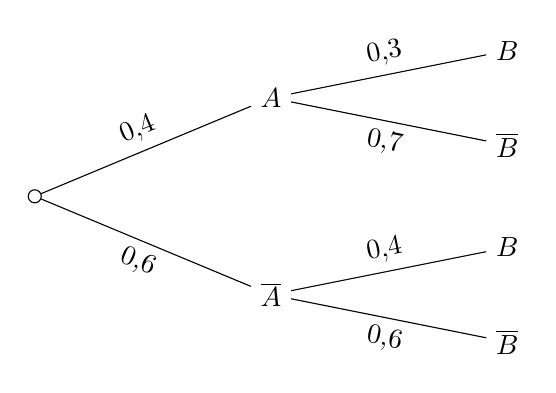
\begin{tikzpicture}[
					grow=right, 
					level distance=3cm, 
					sibling  distance=2.5cm,
					level 2/.style={sibling distance=1.2cm}, 
					ethicknode/.style={scale=0.9}] 
				 \node [draw,circle,scale=0.5] {}
					 child {node{$\overline{A}$}
					child {node{$\overline{B}$} 
					edge  from parent[sloped] node[below] {$0{,}6$}
				 }
					child {node{$B$} 
					edge from parent[sloped]  node[above] {$0{,}4$}
				 }
					edge from parent[sloped]  node[below] {$0{,}6$}
				} 
					child  {node{$A$}
					 child {node{$\overline{B}$}
					 edge from parent[sloped] node[below] {$0{,}7$}
				 }
					child  {node{$B$}
					edge from parent[sloped] node[above] {$0{,}3$} 
				} 
					edge from parent[sloped]  node[above] {$0{,}4$}
					}; 
			\end{tikzpicture}
	\end{center}
	Xác suất của biến cố  $B$ là
	 \choice
		 {$\mathrm{P}(B)=0{,}4\cdot0{,}3$}
		 {$\mathrm{P}(B)=0{,}6\cdot0{,}4$}
		{\True  $\mathrm{P}(B)=0{,}4\cdot0{,}3+0{,}6\cdot0{,}4$}
		{$\mathrm{P}(B)=0{,}4\cdot0{,}3-0{,}6\cdot0{,}4$} 
	\loigiai{Xác suất  để $B$ xảy ra là \\
	$\mathrm{P}(B) = \mathrm{P}(A).\mathrm{P}(B|A)  + \mathrm{P}(\overline{A}).\mathrm{P}(B|\overline{A}) = 0{,}4 \cdot 0{,}3 + 0{,}6 \cdot 0{,}4 = 0{,}12 + 0{,}24 = 0{,}36$.
	 }
\end{ex}

% nguồn: Lop_12_Dai_so_Chuong_6
\begin{ex}%[2D6H2-2]%[ma:4b68f385]
	Cho hai biến cố $A$, $B$ thỏa  mãn $P(A)=0{,}3$; $P(B\mid A)=0{,}4$; $P\left(B\mid\overline{A}\right)=0{,}5$. Khi đó, $P(B)$ bằng
	 \choice
		{\True  $0{,}47$}
		{$0{,}06$} 
		 {$0{,}27$}
		{$0{,}43$} 
	\loigiai{Ta  có $P\left(\overline{A}\right)=1-P(A)=0{,}7$.\\
	 Suy ra $P(B)=P(A)\cdot P(B\mid A)+P\left(\overline{A}\right)\cdot P\left(B\mid \overline{A}\right)=0{,}47$.}
\end{ex}

% nguồn: Lop_12_Dai_so_Chuong_6
\begin{ex}%[2D6H2-2]%[ma:8cdd7535]
	Cho hai biến cố $A$, $B$ với $\mathrm{P}\left(B\right)=0{,}6$, $\mathrm{P}\left(A\mid B\right)=0{,}7$ và $\mathrm{P}\left(A\mid  \overline{B}\right)=0{,}4$. Khi đó, $\mathrm{P}\left(A\right)$ bằng
	\choice 
		 {$0{,}7$}
		 {$0{,}4$}
		{\True  $0{,}58$}
		 {$0{,}52$}
	\loigiai{ 
		Ta có $\mathrm{P}\left(\overline{B}\right)=1-\mathrm{P}\left(B\right)=1-0{,}6=0{,}4$.\\ 
		Theo công  thức xác suất toàn phần ta được
		\[\mathrm{P}\left(A\right)=\mathrm{P}\left(B\right)\cdot\mathrm{P}\left(A\mid B\right)+\mathrm{P}\left(\overline{B}\right)\cdot\mathrm{P}\left(A\mid \overline{B}\right)=0{,}6\cdot 0{,}7+0{,}4\cdot  0{,}4=0{,}58.\]
	 }
\end{ex}

% nguồn: Lop_12_Dai_so_Chuong_6
\begin{ex}%[2D6H2-2]%[ma:f5a246e9]
	Cho $A$, $B$ là hai biến cố. Biết $\mathrm{P}(B)=0{,}2$. Nếu $B$ không xảy ra thì thỉ lệ $A$ xảy ra là $2\%$. Nếu $B$ xảy ra thì tỉ lệ $A$ xảy ra $4\%$. Xác suất của biến  cố $A$ là bao nhiêu?
	 \choice
		{$0{,}018$} 
		{$0{,}036$} 
		{$0{,}028$} 
		{\True  $0{,}024$}
	\loigiai{ 
		Ta có  $\mathrm{P}\left(B\right)=0{,}2\Rightarrow \mathrm{P}\left(\overline{B}\right)=0{,}8$.\\
		Vì $B$ xảy ra thì tỉ lệ $A$ sảy ra $4\%$  nên $\mathrm{P}\left(A\mid B\right)=0{,}04$.\\
		Tương tự ta cũng có  $\mathrm{P}\left(A\mid \overline{B}\right)=0{,}02$. Theo công thức xác suất toàn phần ta có
		 \[\mathrm{P}\left(A\right)=\mathrm{P}\left(B\right)\cdot\mathrm{P}\left(A\mid B\right)+\mathrm{P}\left(\overline{B}\right)\cdot\mathrm{P}\left(A\mid \overline{B}\right)=0{,}2\cdot0{,}04+0{,}8\cdot0{,}02=0{,}024.\]
	 }
\end{ex}

% nguồn: Lop_12_Dai_so_Chuong_6
\begin{ex}%[2D6H2-2]%[ma:46320bae]
	Cho hai biến cố $A$, $B$ thỏa mãn $\mathrm{P}\left(\overline{B}\right)=0{,}2$; $\mathrm{P}\left(A\mid B\right)=0{,}5$; $\mathrm{P}\left( A\mid \overline{B}\right)=0{,}3$. Khi  đó, $\mathrm{P}\left(A\right)$ bằng
	\choice 
		 {\True $0{,}46$}
		{$0{,}34$} 
		 {$0{,}15$}
		{$0{,}31$} 
	\loigiai{ 
		 Ta có $\mathrm{P}\left(B\right)=1-\mathrm{P}\left(\overline{B}\right)=0{,}8$.\\
		Theo công thức xác  suất toàn phần, ta có
		 \[\mathrm{P}\left(A\right)=\mathrm{P}\left(B\right)\cdot\mathrm{P}\left(A\mid B\right)+\mathrm{P}\left(\overline{B}\right)\cdot\mathrm{P}\left(A\mid \overline{B}\right)=0{,}8\cdot0{,}5+0{,}2\cdot0{,}3=0{,}46.\]
	 }
\end{ex}

% nguồn: Lop_12_Dai_so_Chuong_6
\begin{ex}%[2D6H2-2]%[ma:0e6d9beb]
	Cho hai biến cố ngẫu nhiên $A$ và $B$  có $\mathrm{P}(A)=0{,}3$; $\mathrm{P}(B)=0{,}6$; $\mathrm{P}(A\mid B)=0{,}5$. Xác suất của $B$ với điểu kiện $A$ là
	 \choice
		{$0{,}3$} 
		{$\dfrac{3}{5}$} 
		 {$\dfrac{1}{2}$}
		{\True  $1$}
	 \loigiai{
		Ta  có $\mathrm{P}(B \mid A)=\dfrac{\mathrm{P}(A \mid B) \mathrm{P}(B)}{\mathrm{P}(A)}=\dfrac{0{,}5 \cdot 0{,}6}{0{,}3}=1$.
	 }
\end{ex}

% nguồn: Lop_12_Dai_so_Chuong_6
\begin{ex}%[2D6H2-2]%[ma:e3687de2]
	Cho hai biến cố  $A$ và $B$, với $\mathrm{P}(B)=0{,}8$, $\mathrm{P}(A|B)=0{,}7$, $\mathrm{P}(A\overline{B})=0{,}15$. Tính $\mathrm{P}(A)$ kết
	quả bằng 
	 \choice
		 {$0{,}25$}
		{\True  $0{,}71$}
		 {$0{,}55$}
		 {$0{,}5$}
	\loigiai{Áp dụng công thức xác suất  toàn phần, ta có $$\mathrm{P}(A)=\mathrm{P}(AB)+\mathrm{P}(A\overline{B})=\mathrm{P}(A|B)\cdot \mathrm{P}(B)+\mathrm{P}(A\overline{B})=0{,}7\cdot0{,}8+0{,}15=0{,}71.$$}
\end{ex}

% nguồn: Lop_12_Dai_so_Chuong_6
\begin{ex}%[2D6H2-2]%[ma:15160c14]
	Cho hai biến cố ngẫu  nhiên $A$ và $B$ có $\mathrm{P}(A\mid B)=\mathrm{P}(A)$. Tỉ số $\dfrac{\mathrm{P}(B)}{\mathrm{P}(B\mid A)}$ là
	 \choice
		{\True  $1$}
		{$\dfrac{1}{2}$} 
		 {$0$}
		{$2$} 
	\loigiai{ 
		Ta có $\dfrac{P(B)}{P(B  \mid A)}=\dfrac{P(A)}{P(A \mid B)}=1$.
	 }
\end{ex}

% nguồn: Lop_12_Dai_so_Chuong_6
\begin{ex}%[2D6H2-2]%[ma:0532ee14]
	 Cho hai biến cố $A$, $B$ thỏa mãn $\mathrm{P}(A)=\dfrac{2}{5}$; $\mathrm{P}(B\mid A)=\dfrac{1}{3}$. Tính $\mathrm{P}\left(A\cap\overline{B}\right)$.
	 \choice
		 {$\dfrac{3}{8}$}
		 {$\dfrac{2}{15}$}
		{\True  $\dfrac{4}{15}$}
		{$\dfrac{4}{19}$} 
	 \loigiai{
	Ta có $\mathrm{P}\left(A\cap\overline{B}\right)=\mathrm{P}(A)\mathrm{P}\left(\overline{B}\mid A\right)=\mathrm{P}(A)[1-\mathrm{P}\left(B\mid  A\right)]=\dfrac{4}{15}$.
	 }
\end{ex}

% nguồn: Lop_12_Dai_so_Chuong_6
\begin{ex}%[2D6H2-2]%[ma:6ec32641]
	Cho hai biến cố $A$, $B$ với $\mathrm{P}\big(B\big)=0{,}6$;  $\mathrm{P}\big(A \mid B\big)=0{,}7$ và $\mathrm{P}\big(A \mid \overline{B}\big)=0{,}4$. Khi đó, $\mathrm{P}(A)$ bằng
	 \choice
		{$0{,}7$} 
		 {$0{,}4$}
		{\True  $0{,}58$}
		{$0{,}52$} 
	 \loigiai{
		Ta  có $\mathrm{P}\big(\overline{B}\big)=1-\mathrm{P}(B)=1-0{,}6=0{,}4$.\\
		Theo công thức xác suất toàn phần,  ta có
		\[\mathrm{P}\big(A\big)=\mathrm{P}(B) \cdot \mathrm{P}\big(A \mid B\big)+\mathrm{P}\big(\overline{B}\big) \cdot \mathrm{P}\big(A \mid \overline{B}\big)=0{,}6 \cdot 0{,}7+0{,}4 \cdot  0{,}4=0{,}58.\]
	 }
\end{ex}

% nguồn: Lop_12_Dai_so_Chuong_6
\begin{ex}%[2D6H2-2]%[ma:3e239863]
	 Cho 2 biến cố $A$ và $B$. Biết $\mathrm{P}(A\mid B)=0{,}8$; $\mathrm{P}(A\mid \overline{B})=0{,}3$; $\mathrm{P}(B)=0{,}4$. Giá trị $\mathrm{P}(A)$ bằng
	 \choice
		 {$0{,}04$}
		{\True  $0{,}5$}
		{$0{,}1$} 
		 {$0{,}55$}
	\loigiai{Ta có $\mathrm{P}(\overline{B})=1-\mathrm{P}(B)=0{,}6$.\\ 
	Áp dụng công thức xác suất toàn phần ta có $$\mathrm{P}(A)=\mathrm{P}(A\mid B)\cdot  \mathrm{P}(B)+\mathrm{P}(A\mid \overline{B})\cdot \mathrm{P}(\overline{B})=0{,}8\cdot 0{,}4+0{,}3\cdot 0{,}6=0{,}5.$$}
\end{ex}

% nguồn: Lop_12_Dai_so_Chuong_6
\begin{ex}%[2D6H2-2]%[ma:6c5758b2]
	Cho hai biến cố $A$ và $B$.  Biết $\mathrm{P}\left(B\right)=0{,}01$; $\mathrm{P}\left(A\mid B\right)=0{,}7$; $\mathrm{P}\left(A\mid \overline{B}\right)=0{,}09$. Khi đó $\mathrm{P}\left(A\right)$ bằng
	\choice 
		{$0{,}0079$} 
		 {\True $0{,}0961$}
		{$0{,}0916$} 
		 {$0{,}0970$}
	\loigiai{ 
		Ta có $\mathrm{P}\left(B\right)=0{,}01\Rightarrow \mathrm{P}\left(\overline{B}\right)=1-0{,}01=0{,}99$.\\ 
		Theo  công thức xác suất toàn phần, ta có
		\[\mathrm{P}\left(A\right)=\mathrm{P}\left(B\right)\mathrm{P}\left(A\mid  B\right)+\mathrm{P}\left(\overline{B}\right)\mathrm{P}\left(A\mid \overline{B}\right)=0{,}01\cdot0{,}7+0{,}99\cdot0{,}09=0{,}0961.\]
	 }
\end{ex}

% nguồn: Lop_12_Dai_so_Chuong_6
\begin{ex}%[2D6H2-2]%[ma:198b5672]
	Có $2$ xạ thủ loại I và $8$ xạ thủ loại II, xác suất bắn trúng đích của  các loại xạ thủ loại I là $0{,}9$ và loại II là $0{,}7$. Chọn ngẫu nhiên ra một xạ thủ và xạ thủ đó bắn một viên đạn. Tìm xác suất để viên đạn đó trúng đích.
	 \choice
		{\True $0{,}74$} 
		 {$0{,}86$}
		 {$0{,}56$}
		{$0{,}68$} 
	 \loigiai{
		Gọi $A$ là biến cố \lq\lq Viên đạn trúng đích\rq\rq; $B$ là  biến cố \lq\lq Chọn xạ thủ loại I bắn\rq\rq.\\
		Ta có $\mathrm{P}\left(B\right)=\dfrac{2}{10}=0{,}2$; $  \mathrm{P}\left(A\mid B\right)=0{,}9$; $ \mathrm{P}\left(\overline{B}\right)=1-0{,}2=0{,}8$; $ \mathrm{P}\left(A\mid \overline{B}\right)=0{,}7$.\\
		Theo công thức xác suất toàn  phần ta được
		\[\mathrm{P}\left(A\right)=\mathrm{P}\left(B\right)\mathrm{P}\left(A\mid  B\right)+\mathrm{P}\left(\overline{B}\right) \mathrm{P}\left(A\mid \overline{B}\right)= 0{,}2\cdot0{,}9+0{,}8\cdot0{,}7=0{,}74.\]
	} 
\end{ex}

% nguồn: Lop_12_Dai_so_Chuong_6
\begin{ex}%[2D6H2-2]%[ma:62edbfed]
	Hai máy tự động sản xuất cùng một loại chi tiết, trong đó máy $I$ sản xuất $35\%$, máy $II$ sản xuất $65\%$ tổng sản lượng. Tỉ lệ phế phẩm của các máy lần lượt là $0{,}3\%$ và $0{,}7\%$. Chọn  ngẫu nhiên $1$ sản phẩm từ kho. Tính xác suất để chọn được phế phẩm?
	\choice 
		 {\True $0{,}0056$}
		 {$0{,}0065$}
		 {$0{,}065$}
		 {$0{,}056$}
	 \loigiai{
		Gọi 
		\begin{itemize}
			\item $A$ là biến cố chọn được sản phẩm do máy  $I$ sản xuất.
			\item $B$ là biến cố chọn được sản phẩm do  máy $II$ sản xuất.
			 \item $C$ là biến cố chọn được phế phẩm.
		\end{itemize}
		Theo  đề bài, ta có
		\begin{itemize}
			\item $P(A)=35\%=0{,}35$ (xác suất máy $I$ sản  xuất).
			\item $P(B)=65\%=0{,}65$ (xác suất máy $II$  sản xuất).
			\item $P(C\mid A)=0{,}3\%=0{,}003$ (xác suất sản phẩm là phế  phẩm nếu do máy $I$ sản xuất).
			\item $P(C\mid B)=0{,}7\%=0{,}007$ (xác suất sản phẩm là phế phẩm nếu  do máy $II$ sản xuất).
		\end{itemize}
		\begin{center}
			\begin{tikzpicture}[scale=.5,font=\footnotesize,line join=round,line cap=round,>=stealth]
					\coordinate (O)  at (2,-1);
					\begin{scope}[ethicknode/.style={circle,draw,fill=red!10}]
						\node (D2)  at (9,3) {$A$};
						\node (D3) at  (9,-5) {$B$};
						\node (B3) at (16,5)  {$C$};
						\node (B4) at (16,1)  {$\overline{C}$};
						 \node (B5) at (16,-3) {$C$};
						\node (B6)  at (16,-7) {$\overline{C}$};
					\end{scope}
					 \node[right=0.8cm of B3] {Phế phẩm};
					\node[right=0.8cm of B4] {}; 
					\node[right=0.8cm of B5] {Phế  phẩm};
					 \node[right=0.8cm of B6] {};
					\draw[->] (O)--(D2)  node[midway,above] {$0{,}35$};
					\draw[->] (O)--(D3) node[midway,below]  {$0{,}65$};
					 \draw[->] (D2)--(B3) node[midway,above] {$0{,}3\%$};
					 \draw[->] (D2)--(B4) node[midway,below] {};
					\draw[->] (D3)--(B5) node[midway,above] {$0{,}7\%$}; 
					\draw[->]  (D3)--(B6) node[midway,below] {};
				\end{tikzpicture}
		\end{center}
		Ta cần tìm  xác suất để chọn được phế phẩm, tức là $P(C)$.\\
		Áp dụng công thức  xác suất toàn phần ta có
		\begin{align*}
			P(C) &= P(C\mid A) \cdot P(A) + P(C\mid B) \cdot P(B) \\ 
			&=  0{,}003 \cdot 0{,}35 + 0{,}007 \cdot 0{,}65 \\
			&= 0{,}00105 +  0{,}00455 \\
			&= 0{,}0056. 
		\end{align*}
		Vậy xác suất để chọn được phế  phẩm là $0{,}0056$.
	} 
\end{ex}

% nguồn: Lop_12_Dai_so_Chuong_6
\begin{ex}%[2D6H2-2]%[ma:ab8f92dd]
	Cho hai biến cố $A$ và $B$, với $\mathrm{P}(B)=0{,}4$; $\mathrm{P}\left(A\mid B\right)=0{,}5$; $\mathrm{P}\left(A\mid \overline{B}\right)=0{,}3$. Tính  $\mathrm{P}(A)$.
	 \choice
		 {$0{,}2$}
		{\True $0{,}38$} 
		{$0{,}8$} 
		 {$0{,}12$}
	\loigiai{ 
	Ta có 
	\[\mathrm{P}(A)=\mathrm{P}(B)\cdot\mathrm{P}\left(A\mid B\right)+\mathrm{P}\left(\overline{B}\right)\cdot\mathrm{P}\left(A\mid \overline{B}\right)=0{,}4\cdot0{,}5+0{,}6\cdot0{,}3 = 0{,}38.\] 
	 }
\end{ex}

% nguồn: Lop_12_Dai_so_Chuong_6
\begin{ex}%[2D6V2-2]%[ma:c166d968]
	Một trạm chỉ phát hai tín hiệu $A$ và $B$ với xác suất tương ứng $0{,}85$ và $0{,}15$ do có  nhiễu trên đường truyền nên $\dfrac{1}{7}$ tín hiệu $A$ bị méo và thu được như tín hiệu $B$; còn $\dfrac{1}{8}$ tín hiệu $B$ bị méo thành và thu được như $A$. Xác suất thu được tín hiệu $A$ là
	 \choice
		{$\dfrac{963}{1120}$} 
		{$\dfrac{283}{1120}$} 
		{\True $\dfrac{837}{1120}$} 
		 {$\dfrac{157}{1120}$}
	\loigiai{ 
		Gọi $A$  là biến cố \lq\lq Phát tín hiệu $A$\rq\rq.\\
		 Gọi $B$ là biến cố \lq\lq Phát tín hiệu $B$\rq\rq.\\
		Gọi $T_A$ là biến cố \lq\lq Phát được tín  hiệu $A$\rq\rq.\\
		Gọi $T_B$ là  biến cố \lq\lq Phát được tín hiệu $B$\rq\rq.\\
		Với $\mathrm{P}\left(T_A \right)=\mathrm{P}\left(A\right)\cdot\mathrm{P}\left(T_A\mid  A\right)+\mathrm{P}\left(B\right)\cdot\mathrm{P}\left(T_A\mid B\right)$\\
		Ta  có $\mathrm{P}\left(A\right)=0{,}85$;
		 $\mathrm{P}\left(T_B\mid A\right)=\dfrac{1}{7}$\\
		$\Rightarrow \mathrm{P}\left(T_A\mid A\right)=1-\dfrac{1}{7}=\dfrac{6}{7}$; $ \mathrm{P}\left(B\right)=0{,}15$; $\mathrm{P}\left(T_A\mid  B\right)=\dfrac{1}{8}$.\\
		Do đó $\mathrm{P}\left(T_A \right)=\mathrm{P}\left(A\right)\cdot\mathrm{P}\left(T_A\mid  A\right)+\mathrm{P}\left(B\right)\cdot\mathrm{P}\left(T_A\mid B\right)=0{,}85\cdot\dfrac{6}{7}+0{,}15\cdot\dfrac{1}{8}=\dfrac{837}{1\,120}$.
	} 
\end{ex}

% nguồn: Lop_12_Dai_so_Chuong_6
\begin{ex}%[2D6V2-2]%[ma:2dc5d4f7]
	Hộp thứ nhất có $4$ viên bi xanh và $6$ viên bi đỏ. Hộp thứ hai có $3$ viên bi xanh và $7$ viên bi đỏ. Các viên bi có cùng kích thước và khối lượng. Lấy ra ngẫu nhiên  $1$ viên bi từ hộp thứ nhất chuyển sang hộp thứ hai. Sau đó lại lấy ra ngẫu nhiên đồng thời $2$ viên bi từ hộp thứ hai. Xác suất để lấy ra hai viên bi đỏ ở hộp thứ hai là
	\choice 
		{\True  $\dfrac{126}{275}$}
		 {$\dfrac{105}{275}$}
		{$\dfrac{110}{275}$} 
		 {$\dfrac{140}{275}$}
	 \loigiai{
		Gọi $A$ là biến cố \lq\lq Lấy được $1$ viên bi màu xanh ở hộp thứ nhất\rq\rq \, và $B$ là biến cố \lq\lq Lấy được  $2$ viên bi màu đỏ ở hộp thứ hai\rq\rq.\\
		Khi đó ta có $\mathrm{P}\left(A\right)=\dfrac{2}{5}$; $\mathrm{P}\left(B\mid A\right)= \dfrac{\mathrm{C}_7^2}{\mathrm{C}_{11}^2}=\dfrac{21}{55}$ (vì hộp thứ  hai có $4$ bi xanh và $7$ bi đỏ).\\
		Suy ra $\mathrm{P}\left(\overline{A}\right)=1-\mathrm{P}\left(A\right)=\dfrac{3}{5}$; $\mathrm{P}\left(B \mid \overline{A}\right)=\dfrac{\mathrm{C}_8^2}{\mathrm{C}_{11}^2}=\dfrac{28}{55}$ (vì hộp thứ hai  có $3$ bi xanh và $8$ bi đỏ).\\
		Áp  dụng công thức xác suất toàn phần ta được
		\[\mathrm{P}\left(B\right)=\mathrm{P}\left(A\right)\cdot\mathrm{P}\left(B\mid A\right)+\mathrm{P}\left(\overline{A}\right)\cdot\mathrm{P}\left(B\mid\overline{A}\right)=\dfrac{2}{5}\cdot\dfrac{21}{55}+\dfrac{3}{5}\cdot\dfrac{28}{55}=\dfrac{126}{275}.\] 
	} 
\end{ex}


%%%%%%%%%%%%%%%% ĐÚNG/SAI %%%%%%%%%%%%%%%%

% nguồn: Lop_12_Dai_so_Chuong_6
\begin{ex}%[2D6N2-2]%[ma:8ef5dafa]
	Cho sơ  đồ hình cây như hình vẽ dưới đây
	\begin{center}
		\begin{tikzpicture}[line cap=round,line join=round,x=0.6cm,y=0.5cm]
				\coordinate  (O) at (2,-1);
				\begin{scope}[ethicknode/.style={circle,draw,fill=red!10}]
					\node at  (1.3,-1) {$O$};
					\node (A) at (9,2)  {$A$};
					\node  (B) at (9,-4) {$\overline{A}$};
					\node (C)  at (16,4) {$B$};
					\node (D) at (16,0) {$\overline{B}$}; 
					\node (E)  at (16,-2.5) {$B$};
					\node (F) at (16,-6.5)  {$\overline{B}$};
				\end{scope}
				\draw (O) -- (A) --  (C)
					(A)  -- (D)
					(O)  -- (B) -- (E)
					(B) -- (F); 
				\begin{scope}
					\node at  (5,1.5) {$0{,}2$};
					\node at  (12,4) {$0{,}3$};
					\node at (12,-2)  {$0{,}8$};
				\end{scope}
			\end{tikzpicture}
	\end{center}
	 \choiceTF
		{\True  Xác suất của biến cố $A$ là $0{,}2$}
		{Xác suất của biến cố $B$ với điều kiện $A$ không xảy ra  là $0{,}3$}
		{\True Xác suất của biến  cố $\overline{A}$ là $0{,}8$}
		{\True Xác  suất của biến cố $B$ là $0{,}7$}
	 \loigiai{
		\begin{itemchoice}
			\itemch  Xác suất của biến cố $A$ là $\mathrm{P}(A)=0{,}2$.
			\itemch Xác suất của biến cố $B$ với điều kiện $A$  không xảy ra là $\mathrm{P}\big(B \mid \overline{A}\big)=0{,}8$.
			\itemch Xác suất của  biến cố $\overline{A}$ là $\mathrm{P}\big(\overline{A}\big)=1-\mathrm{P}(A)=1-0,2=0{,}8$.
			\itemch Xác suất của  biến cố $B$ là
			\[ 
			 \mathrm{P}(B)=\mathrm{P}(A)\cdot \mathrm{P}(B \mid A)+\mathrm{P}(\overline{A})\cdot \mathrm{P}(B\mid \overline{A})=0{,}2\cdot0{,}3+0{,}8\cdot0{,}8=0,7.
			\] 
		\end{itemchoice}
	} 
\end{ex}

% nguồn: Lop_12_Dai_so_Chuong_6
\begin{ex}%[2D6H2-2]%[ma:61aa8f55]
	Một hộp có $12$ quả bóng màu xanh, $7$ quả bóng màu đỏ; các quả bóng có kích thước và khối lượng như nhau. Lấy ngẫu nhiên lần lượt hai  quả bóng trong hộp, lấy không hoàn lại. Xét các biến cố:
	\begin{itemize}
		\item $A$:  \lq\lq Lần thứ hai lấy được quả màu đỏ\rq\rq.
		 \item $B$: \lq\lq Lần thứ nhất lấy được quả màu xanh\rq\rq.
	\end{itemize}
	 \choiceTF
		{$\mathrm{P}(B)=\dfrac{7}{9}$} 
		{$\mathrm{P}\left(A\cap  B\right)=\dfrac{28}{57}$}
		 {\True $\mathrm{P}\left(A\mid B\right)=\dfrac{7}{18}$}
		 {\True $\mathrm{P}\left(\overline{A}\right)=\dfrac{12}{19}$}
	\loigiai{ 
	\begin{itemchoice}
		\itemch Có  $\mathrm{P}(B)=\dfrac{12}{19}$.
		\itemch  Có $\mathrm{P}\left(A\cap B\right)=\dfrac{12}{19}\cdot\dfrac{7}{18}=\dfrac{14}{57}$.
		\itemch $\mathrm{P}\left(A\mid B\right)=\dfrac{\mathrm{P}\left(A\cap  B\right)}{\mathrm{P}(B)}=\dfrac{7}{18}$.
		 \itemch $\mathrm{P}\left(\overline{A}\right)=\mathrm{P}(B)\cdot\mathrm{P}\left(\overline{A}\mid B\right)+\mathrm{P}\left(\overline{B}\right)\cdot\mathrm{P}\left(\overline{A}\mid \overline{B}\right)=\dfrac{12}{19}\cdot\dfrac{11}{18}+\dfrac{7}{19}+\dfrac{12}{18}=\dfrac{12}{19}$.
	\end{itemchoice}
	} 
\end{ex}

% nguồn: Lop_12_Dai_so_Chuong_6
\begin{ex}%[2D6H2-2]%[ma:ba561123]
	Điểm kiểm tra cuối kì môn Toán của một học sinh phụ thuộc vào việc học sinh đó  có chăm chỉ làm bài tập về nhà hay không. Nếu bạn An chăm chỉ làm bài tập về nhà môn Toán thì xác suất đạt điểm tốt kiểm tra cuối kì là $0{,}9$. Còn nếu bạn An không chăm chỉ làm bài tập về nhà thì xác suất đạt điểm không tốt kiểm tra cuối kì là $0{,}85$. Xác suất An chăm chỉ làm bài tập về nhà môn Toán là $0{,}75$.
	\choiceTF 
		{\True Nếu An chăm chỉ làm bài tập về nhà môn Toán thì xác suất An được điểm không tốt kiểm tra cuối  kì là $0{,}1$}
		{Nếu An không chăm chỉ làm  bài tập về nhà môn Toán thì xác suất An được điểm tốt kiểm tra cuối kì là $0{,}2$}
		{Xác suất để An đạt điểm không tốt  kiểm tra cuối kì là $0{,}35$}
		{\True Xác suất để An đạt điểm  tốt kiểm tra cuối kì là $0{,}7125$}
	\loigiai{ 
		Gọi $A$ là biến cố \lq\lq An chăm chỉ làm bài tập về  nhà môn Toán\rq\rq \, và $B$ là biến cố \lq\lq An đạt điểm tốt kiểm tra cuối kì\rq\rq. Ta có $\mathrm{P}(A)=0{,}75$, $\mathrm{P}\left(\overline{A}\right)=1-0{,}75=0{,}25$.
		\begin{itemchoice}
			\itemch Vì theo giả thiết, nếu bạn An chăm chỉ làm bài tập về nhà môn Toán thì xác suất đạt điểm tốt kiểm tra cuối  kì là $0{,}9$. Vậy, nếu An chăm chỉ làm bài tập về nhà môn Toán thì xác suất An được điểm không tốt kiểm tra cuối kì là
			\[\mathrm{P}\left(\overline{B}\mid  A\right)=1-0{,}9=0{,}1.\]
			\itemch Vì theo giả thiết, nếu bạn An không chăm  chỉ làm bài tập về nhà môn Toán thì xác suất đạt điểm không tốt kiểm tra cuối kì là $0{,}85$. Vậy, nếu An không chăm chỉ làm bài tập về nhà môn Toán thì xác suất An được điểm tốt kiểm tra cuối kì là $\mathrm{P}\left(B\mid \overline{A}\right)=1-0{,}85=0{,}15$.
			\itemch Theo công thức tính xác  suất toàn phần, xác suất để An đạt điểm không tốt kiểm tra cuối kì là
			 \[\mathrm{P}\left(\overline{B}\right)=\mathrm{P}(A)\cdot \mathrm{P}\left(\overline{B}\mid A\right)+\mathrm{P}\left(\overline{A}\right)\cdot \mathrm{P}\left(\overline{B}\mid \overline{A}\right)=0{,}75\cdot 0{,}1+0{,}25\cdot 0{,}85=0{,}2875.\]
			\itemch Theo công thức tính xác  suất toàn phần, xác suất để An đạt điểm tốt kiểm tra cuối kì là
			 \[\mathrm{P}(B)=\mathrm{P}(A)\cdot\mathrm{P}(B\mid A)+\mathrm{P}\left(\overline{A}\right) \cdot\mathrm{P}\left(B\mid \overline{A}\right)=0{,}75\cdot 0{,}9+0{,}25\cdot0{,}15=0{,}7125.\]
			Hoặc  $\mathrm{P}(B)=1-\mathrm{P}\left(\overline{B}\right)=1-0{,}2875=0{,}7125$.
		\end{itemchoice}
	} 
\end{ex}

% nguồn: Lop_12_Dai_so_Chuong_6
\begin{ex}%[2D6H2-2]%[ma:631c0e3f]
	Bạn Ngọc phải thực hiện hai thí nghiệm liên tiếp. Thí nghiệm thứ nhất có xác suất thành công là $0{,}8$. Nếu thí nghiệm thứ nhất thành công thì xác suất thành công của thí nghiệm thứ hai là $0{,}9$. Nếu thí nghiệm thứ nhất không thành công thì xác suất thành công của thí nghiệm thứ hai chỉ là $0{,}5$. Xét các biến cố sau:\\ 
	Gọi $A$ là biến  cố \lq\lq Thí nghiệm thứ nhất thành công\rq\rq.\\
	 Gọi $B$ là biến cố \lq\lq Thí nghiệm thứ hai thành công\rq\rq.\\
	Khi  đó
	 \choiceTF
		 {\True $\mathrm{P}(B\mid A)=0{,}9$}
		{$\mathrm{P}\left(\overline{B}\mid  A\right)=0{,}5$}
		{\True $\mathrm{P}(AB)=0{,}72$} 
		{\True  $\mathrm{P}\left(\overline{A} \overline{B}\right)=0{,}1$}
	\loigiai{ 
		\begin{itemchoice}
			\itemch $\mathrm{P}(B\mid A)$ là xác suất  thí nghiệm thứ $2$ thành công nếu thí nghiệm thứ nhất thành công do đó $\mathrm{P}(B\mid A)=0{,}9$.
			\itemch $\mathrm{P}\left(\overline{B}\mid A \right)=1-\mathrm{P}(B\mid A)=1-0{,}9=0{,}1$. 
			\itemch $\mathrm{P}(AB)=\mathrm{P}(A)\cdot\mathrm{P}(B\mid  A)=0{,}8\cdot0{,}9=0{,}72$.
			\itemch $\overline{A}\overline{B}$ là biến cố \lq\lq Cả hai thí nghiệm đều không  thành công\rq\rq.\\
			Theo giả thiết,  $\mathrm{P}\left(\overline{A}\right)=1-0{,}8=0{,}2$ và $\mathrm{P}\left(\overline{B}\mid \overline{A}\right)=1-\mathrm{P}\left(B\mid \overline{A}\right)=1-0{,}5=0{,}5$.\\
			 Vậy xác suất để cả hai thí nghiệm không thành công là
			\[\mathrm{P}\left(\overline{A}\overline{B}\right)=\mathrm{P}\left(\overline{A}\right)\cdot \mathrm{P}\left(\overline{B}\mid  \overline{A}\right)=0{,}2\cdot 0{,}5=0{,}1.\]
		\end{itemchoice}
	} 
\end{ex}

% nguồn: Lop_12_Dai_so_Chuong_6
\begin{ex}%[2D6H2-2]%[ma:9be6c884]
	Cho sơ đồ hình cây  như hình bên. Khi đó
	\begin{center}
		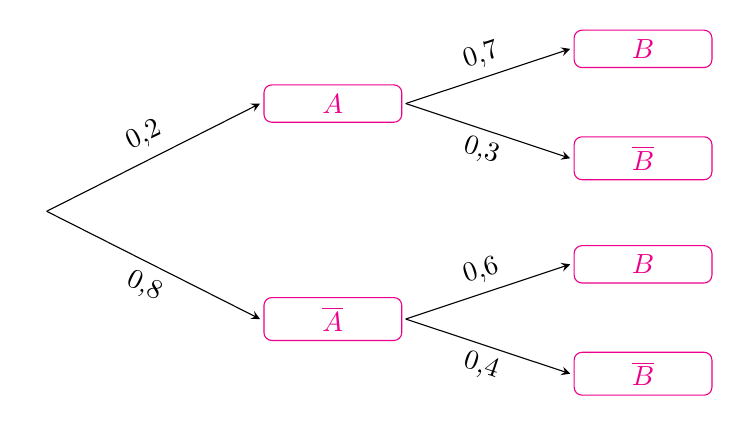
\begin{tikzpicture}
				 \def\gocm{20}
				\def\gocn{10} 
				\def\r{4} 
				\tikzset{s/.style={outer sep=0.5  mm,draw,magenta,rectangle,minimum width=1.75cm,rounded corners=1mm}}
				\path (0,0) node (O){}++(\gocm:\r) node[s](A1){$A$}++(\gocn:\r) node[s](A2){$B$}; 
				\path  (A1)++({-\gocn}:\r) node[s](a2){$\overline{B}$};
				\path (O)++(-\gocm:\r) node[s](B1){$\overline{A}$}++(\gocn:\r)  node[s](B2){$B$};
				\path (B1)++({-\gocn}:\r) node[s](b2){$\overline{B}$}; 
				\foreach \x/\y in  {
					 O/A1,A1/A2,
					 O/B1,B1/B2,
					A1/a2, 
					B1/b2} 
				 \draw[-stealth](\x.east)--(\y.west);
				\path  (O)--(A1.west) node[pos=0.5,above,sloped]{$\mbox{0{,}2}$}
					(O)--(B1.west) node[pos=0.5,below,sloped]{$\mbox{0{,}8}$} 
					(B1.east)--(B2.west) node[pos=0.5,above,sloped]{$\mbox{0{,}6}$} 
					 (A1.east)--(A2.west) node[pos=0.5,above,sloped]{$\mbox{0{,}7}$}
					(A1.east)--(a2.west) node[pos=0.5,below,sloped]{$\mbox{0{,}3}$} 
					 (B1.east)--(b2.west) node[pos=0.5,below,sloped]{$\mbox{0{,}4}$};
			\end{tikzpicture}
	\end{center}
	\choiceTF 
		{\True $\mathrm{P}(B)=\mathrm{P}(A)\cdot  \mathrm{P}(B\mid A)+\mathrm{P}\left(\overline{A} \right) \cdot \mathrm{P}\left(B\mid\overline{A}\right)$}
		 {$\mathrm{P}(B\mid A)=0{,}6$}
		{\True $\mathrm{P}(B)=0{,}62$} 
		{$\mathrm{P}\left(\overline{B}\right)=0{,}4$} 
	\loigiai{ 
		\begin{itemchoice}
			\itemch Công thức xác suất toàn phần $\mathrm{P}(B)=\mathrm{P}(A)\cdot  \mathrm{P}(B\mid A)+\mathrm{P}\left(\overline{A} \right) \cdot \mathrm{P}\left(B\mid\overline{A}\right)$.
			\itemch Dựa vào sơ đồ cây ta có $\mathrm{P}(B\mid A)=0{,}7$. 
			\itemch Xác suất của biến cố $B$ là $\mathrm{P}(B)=0{,}2\cdot 0{,}7+0{,}8\cdot  0{,}6=0{,}62$.
			\itemch Ta có  $\mathrm{P}\left(\overline{B}\right)=1-\mathrm{P}(B)=0{,}38$.
		\end{itemchoice}
	 }
\end{ex}

% nguồn: Lop_12_Dai_so_Chuong_6
\begin{ex}%[2D6H2-2]%[ma:a7ab1ed2]
	Hộp thứ nhất chứa $5$ viên bi vàng, $3$ viên bi xanh. Hộp thứ hai chứa $4$ viên bi vàng, $5$ viên bị xanh và $3$ viên bi đỏ. Lấy ngẫu nhiên $1$ viên bi từ hộp thứ nhất  bỏ vào hộp thứ hai, sau đó lấy ra $2$ viên bi bất kỳ từ hộp thứ hai. Khi đó
	 \choiceTF
		{\True Xác suất để lấy được bi xanh từ hộp thứ nhất là  $\dfrac{3}{8} $}
		 {Xác suất để lấy được bi vàng từ hộp thứ nhất là $\dfrac{5}{7} $}
		{\True Biết rằng lấy được bi màu xanh từ hộp thứ nhất. Xác  suất để lấy được $2$ viên bi khác màu từ hộp thứ hai là $\dfrac{9}{13} $}
		{Xác suất để lấy  được $2$ bi vàng từ hộp thứ hai là $\dfrac{5}{32} $}
	 \loigiai{
		Gọi $A$ là  biến cố lấy được bi xanh từ hộp thứ nhất.
		\begin{itemchoice}
			\itemch Ta  có $\mathrm{P}(A)=\dfrac{3}{8} $.
			\itemch Ta có  $\overline{A}$ là biến cố lấy được bi vàng từ hộp thứ nhất, suy ra $\mathrm{P}\left(\overline{A}\right)=\dfrac{5}{8} $.
			\itemch Gọi $B_{1} $ là biến cố lấy được $2$ bi khác màu  từ hộp thứ hai.\\
			 Ta có $\mathrm{P}(B_{1} \mid A)=\dfrac{\mathrm{C}_4^1 \cdot \mathrm{C}_6^1 +\mathrm{C}_4^1 \cdot \mathrm{C}_3^1 +\mathrm{C}_3^1 \cdot \mathrm{C}_6^1}{\mathrm{C}_{13}^{2}} =\dfrac{9}{13} $.\\
			\itemch  Gọi $B_{2} $ là biến cố lấy được 2 bi vàng từ hộp thứ hai.\\
			Ta có $\mathrm{P}(B_{2})=\mathrm{P}(A) \cdot \mathrm{P}(B_{2} \mid A)+\mathrm{P}\left(\overline{A}\right) \cdot \mathrm{P}\left(B_{2} \mid \overline{A} \right)=\dfrac{3}{8} \cdot  \dfrac{\mathrm{C}_{4}^{2}}{\mathrm{C}_{13}^{2}} +\dfrac{5}{8} \cdot \dfrac{\mathrm{C}_5^2}{\mathrm{C}_{13}^{2}} =\dfrac{17}{156}.$
		\end{itemchoice}
	 }
\end{ex}

% nguồn: Lop_12_Dai_so_Chuong_6
\begin{ex}%[2D6H2-2]%[ma:d6a9cfe3]
	Có hai chiếc hộp. Hộp thứ nhất có $5$ viên bi xanh và $7$ viên bi đỏ. Hộp thứ hai có $6$ viên bi xanh và $8$ viên bi đỏ. Các viên bi có cùng kích thước và khối lượng. Lấy ra ngẫu nhiên $1$ viên bi từ hộp thứ nhất chuyển sang hộp thứ hai. Sau đó lại lấy ra  ngẫu nhiên đồng thời $2$ viên bi từ hộp thứ hai. Gọi $A$ là biến cố \lq\lq Lấy được $1$ viên bi màu xanh ở hộp thứ nhất\rq\rq \,và $B$ là biến cố \lq\lq Lấy được $2$ viên bi màu đỏ ở hộp thứ hai\rq\rq.
	\choiceTF 
		{$\mathrm{P}\left(\overline{A}\right)=\dfrac{5}{12}  $}
		{$\mathrm{P}(B\mid A)=\dfrac{1}{15} $} 
		 {\True $\mathrm{P}\left(B\mid \overline{A}\right)=\dfrac{12}{35} $}
		{\True $\mathrm{P}(B)=\dfrac{14}{45} $} 
	\loigiai{ 
		\begin{itemchoice}
			\itemch Ta có $\mathrm{P}(A)=\dfrac{5}{12}  \Rightarrow \mathrm{P}\left(\overline{A}\right)=1-\mathrm{P}(A)=\dfrac{7}{12} $.
			\itemch Nếu $A$ xảy ra thì khi đó hộp  hai chứa $7$ bi xanh và $8$ bi đỏ.\\
			Chọn hai bi bất kì từ hộp hai  có $\mathrm{C}_{15}^2 $ cách. Chọn hai bi đỏ từ hộp hai có $\mathrm{C}_8^2 $ cách.\\
			Suy ra: $\mathrm{P}(B\mid A)=\dfrac{\mathrm{C}_{8}^2}{\mathrm{C}_{15}^2 }=\dfrac{4}{15} $. 
			\itemch Nếu $A$ không xảy ra thì khi đó  hộp hai chứa $6$ bi xanh và $9$ bi đỏ.\\
			Chọn hai bi bất kì từ hộp hai có $\mathrm{C}_{15}^2 $ cách. Chọn hai bi đỏ từ hộp hai có $\mathrm{C}_9^2  $ cách.\\
			Suy ra $\mathrm{P}\left(B\mid \overline{A}\right)=\dfrac{\mathrm{C}_{9}^2}{\mathrm{C}_{15}^2} =\dfrac{12}{35}  $.
			\itemch Áp dụng công  thức xác suất toàn phần
			\[\mathrm{P}(B)=\mathrm{P}(A)\cdot\mathrm{P}(B\mid A)+\mathrm{P}(\overline{A})\cdot\mathrm{P}\left(B\mid\overline{A}\right)=\dfrac{5}{12} \cdot\dfrac{4}{15} +\dfrac{7}{12}  \cdot\dfrac{12}{35} =\dfrac{14}{45} .\]
		\end{itemchoice}
	} 
\end{ex}

% nguồn: Lop_12_Dai_so_Chuong_6
\begin{ex}%[2D6H2-2]%[ma:ea46bd2d]
	Cho $A$ và $B$ là hai biến cố  của cùng phép thử, biết rằng $\mathrm{P}(B)=0{,}3$;\break $\mathrm{P}(A\mid B)=0{,}01$ và $\mathrm{P}\left(A\mid \overline{B}\right)=0{,}02$. Khi đó
	 \choiceTF
		 {$\mathrm{P}\left(\overline{B}\right)=0{,}07$}
		{\True Công thức xác suất toàn phần là $\mathrm{P}(A)=\mathrm{P}(B) \cdot  \mathrm{P}(A\mid B)+\mathrm{P}\left(\overline{B} \right) \cdot \mathrm{P}\left(A\mid \overline{B} \right)$}
		{Công thức xác suất toàn phần là $\mathrm{P}(A)=\mathrm{P}(\overline{B})  \cdot \mathrm{P}(A\mid B)+\mathrm{P}(B) \cdot \mathrm{P}\left(A\mid \overline{B} \right)$}
		{\True $\mathrm{P}(A)=0{,}017$} 
	 \loigiai{
		\begin{itemchoice}
			 \itemch $\mathrm{P}\left(\overline{B}\right)=1-\mathrm{P}(B)=1-0{,}3=0{,}7$.
			\itemch Công thức xác suất toàn phần là $\mathrm{P}(A)=\mathrm{P}(B)\mathrm{P}(A\mid  B)+\mathrm{P}\left(\overline{B}\right)\mathrm{P}(A\mid \overline{B})$.
			\itemch Công thức $\mathrm{P}(A)=\mathrm{P}(B)  \cdot \mathrm{P}(A\mid B)+\mathrm{P}\left(\overline{B}\right) \cdot \mathrm{P}\left(A\mid \overline{B}\right)$.
			\itemch $\mathrm{P}(A)=\mathrm{P}(B) \cdot \mathrm{P}(A\mid B)+\mathrm{P}\left(\overline{B}\right) \cdot \mathrm{P}\left(A\mid \overline{B}\right)$$=0{,}3\cdot 0{,}01+0{,}7\cdot 0{,}02=0{,}017$. 
		\end{itemchoice}
	 }
\end{ex}

% nguồn: Lop_12_Dai_so_Chuong_6
\begin{ex}%[2D6H2-2]%[ma:a1047815]
	Hình dạng hạt của đậu Hà Lan có hai kiểu hình: hạt trơn và hạt nhăn, có hai gene ứng với hai kiểu hình này là gene trội $B$ và  gene lặn $b$. Khi cho lai hai cây đậu Hà Lan, cây con lấy ngẫu nhiên một cách độc lập một gene từ cây bố và một gene từ cây mẹ để hình thành một cặp gene. Giả sử cây bố và cây mẹ được chọn ngẫu nhiên từ một quần thể các cây đậu Hà Lan, ở đó tỉ lệ cây mang kiểu gene $bb$, $Bb$ tương ứng là $40\% $ và $60\% $. Khi đó
	 \choiceTF
		{Xác suất để cây con lấy gene $b$ từ cây bố với điều  kiện cây bố có kiểu gene $bb$ là $0{,}5$}
		{\True Xác suất để cây con lấy gene $b$ từ cây bố với điều kiện cây bố có kiểu  gene $Bb$ là $0{,}5$}
		{Xác suất để cây con  lấy gene $b$ từ cây bố là $0{,}6$}
		{\True Xác suất để  cây con có kiểu gene $bb$ là $0{,}49$}
	\loigiai{ 
		Gọi $A$ là biến cố: \lq\lq Cây bố  có kiểu gene $bb$\rq\rq;\\
		$M$ là biến cố: \lq\lq Cây con lấy gene $b$ từ  cây bố\rq\rq;\\
		$N$ là  biến cố: \lq\lq Cây con lấy gene $b$ từ cây mẹ\rq\rq;\\ $E$ là biến cố: \lq\lq Cây con có kiểu gene $bb$\rq\rq.\\
		Theo giả thiết $M$ và $N$ độc lập nên $\mathrm{P}(E)=\mathrm{P}(M)\cdot\mathrm{P}(N)$.\\ 
		Ta áp dụng công thức xác suất toàn phần $\mathrm{P}(M)=\mathrm{P}(A)\cdot\mathrm{P}(M\mid A)+\mathrm{P}\left(\overline{A}\right) \cdot  \mathrm{P}\left(M\mid \overline{A}\right)\quad(*)$.\\
		Suy ra  $\mathrm{P}(A)=0{,}4$; $ \mathrm{P}\left(\overline{A}\right)=0{,}6$.
		\begin{itemchoice}
			\itemch $\mathrm{P}\left(M \mid A \right)$ là xác suất để cây con lấy gene $b$ từ cây bố với điều kiện  cây bố có kiểu gene $bb$. Do đó $\mathrm{P}(MA)=1$.
			\itemch $\mathrm{P}(M\mid \overline{A})$ là xác suất để cây con lấy gene $b$ từ cây bố với điều kiện cây bố có kiểu gene $Bb$. Do đó  $\mathrm{P}(M\mid \overline{A})=\dfrac{1}{2} $.
			\itemch Thay vào $(*)$ ta được $\mathrm{P}(M)=0{,}4\cdot  1+0{,}6\cdot 0{,}5=0{,}4+0{,}3=0{,}7$.
			\itemch Tương tự  tính được $\mathrm{P}(N)=0{,}7$. Vậy $\mathrm{P}(E)=\mathrm{P}(M)\cdot\mathrm{P}(N)=0{,}7\cdot0{,}7=0{,}49$.\\
			Từ kết quả trên suy ra trong một quần thể các cây  đậu Hà Lan, ở đó tỉ lệ cây bố và cây mẹ mang kiểu gene $bb$, $Bb$ tương ứng là $40\% $ và $60\% $, thì tỉ lệ cây con có kiểu gene $bb$ là khoảng $49\% $.
		\end{itemchoice}
	} 
\end{ex}

% nguồn: Lop_12_Dai_so_Chuong_6
\begin{ex}%[2D6V2-2]%[ma:9bff539b]
	Có hai chiếc hộp, hộp I có $7$ quả bóng màu đỏ và $4$ quả bóng màu vàng, hộp II có $5$ quả bóng màu đỏ và $6$ quả bóng màu vàng, các quả bóng có cùng kích thước và khối  lượng. Lấy ngẫu nhiên một quả bóng từ hộp I bỏ vào hộp II. Sau đó, lấy ra ngẫu nhiên một quả bóng từ hộp II. Xét tính đúng sai của các mệnh đề sau?
	\choiceTF 
		{Xác suất lấy từ hộp II quả bóng màu vàng là $\dfrac{31}{66}$} 
		{Xác suất  lấy được quả bóng màu đỏ từ hộp I bỏ vào hộp II là $\dfrac{4}{11}$}
		{\True Biết lấy  được $1$ quả đỏ từ hộp I bỏ sang hộp II, xác suất để lấy ra quả đỏ từ hộp II là $\dfrac{1}{2}$}
		{\True Xác suất để quả bóng được lấy ra từ hộp II là quả bóng được chuyển từ hộp I sang, biết rằng quả bóng đó có màu vàng (làm tròn kết quả đến  hàng phần trăm) là $0{,}06$}
	\loigiai{ 
		\begin{itemchoice}
			\itemch Gọi $A$ là biến cố: \lq\lq Lấy được quả bóng màu  vàng từ hộp I\rq\rq.\\
			$B$ là biến cố:  \lq\lq Lấy được quả bóng màu vàng từ hộp II\rq\rq. \\
			Vì hộp I có $7$ quả bóng màu đỏ và $4$ quả bóng màu  vàng nên $\mathrm{P}(A)=\dfrac{4}{11}$. \\
			Suy  ra $\mathrm{P}(\overline{A})=1-\mathrm{P}(A)=1-\dfrac{4}{11}=\dfrac{7}{11}$.\\
			Nếu $A$ xảy ra tức là lấy được quả bóng màu vàng từ hộp I rồi  cho sang hộp II thì hộp II có $5$ quả bóng màu đỏ và $7$ quả bóng màu vàng. \\
			Do đó $\mathrm{P}(B  \mid A)=\dfrac{7}{12}$. \\
			Nếu $A$ không xảy ra thì hộp II có $6$ quả bóng màu đỏ và $6$ quả bóng màu  vàng.\\
			Do đó  $\mathrm{P}(B \mid \overline{A})=\dfrac{6}{12}=\dfrac{1}{2}$.\\
			Khi  đó
			\[\mathrm{P}(B)=\mathrm{P}(A) \cdot \mathrm{P}(B \mid A)+\mathrm{P}(\overline{A})\cdot \mathrm{P}(B \mid \overline{A})=\dfrac{4}{11} \cdot \dfrac{7}{12}  + \dfrac{7}{11} \cdot \dfrac{1}{2} = \dfrac{35}{66}.\]
			\itemch Trong hộp I có $7$ quả đỏ,  nên xác suất lấy được quả bóng màu đỏ từ hộp I bỏ vào hộp II là $\dfrac{7}{11}$.
			\itemch Vì lấy được $1$ quả đỏ từ hộp I bỏ sang hộp  II, nên trong hộp II có $6$ quả đỏ.\\
			Xác suất lấy ra quả đỏ từ  hộp II là $\dfrac{1}{2}$.
			\itemch Gọi $C$ là biến cố \lq\lq Lấy ra từ hộp  II là quả bóng được chuyển từ hộp I sang\rq\rq. \\
			$D$ là biến cố \lq\lq Lấy ra từ hộp II là quả bóng  màu vàng\rq\rq. \\
			Ta xét hai  trường hợp
			\begin{itemize}
				\item  Trường hợp $1$: Lấy một quả màu vàng từ hộp I sang hộp II, rồi lấy một quả màu vàng từ hộp II, có $4 \cdot 7 =28$ cách.
				\item Trường hợp $2$: Lấy một quả màu đỏ từ hộp I sang hộp II, rồi lấy một quả màu vàng từ hộp II, có $7 \cdot 6 = 42$  cách.
			\end{itemize}
			Suy ra $n(D)=28+42=70$.  \\
			$C \cap D$: \lq\lq Lấy một quả vàng từ hộp I sang hộp II rồi lấy quả vàng đó từ  hộp II\rq\rq\, do đó $n(C\cap D)= 4 \cdot 1 = 4$.\\
			 Xác suất $\mathrm{P}(C\mid D)=\dfrac{4}{70} \approx 0{,}06$.
		\end{itemchoice}
	} 
\end{ex}

% nguồn: Lop_12_Dai_so_Chuong_6
\begin{ex}%[2D6V2-2]%[ma:760044ae]
	Trong năm học vừa qua, ở trường đại học X, tỉ lệ sinh viên thi trượt môn Toán là $30\%$, thi trượt môn Tâm lý là $22\%$. Trong số các sinh viên trượt môn Toán có $40\%$ sinh  viên trượt môn Tâm lý. Gặp ngẫu nhiên một sinh viên trường X. Sử dụng sơ đồ hình cây để tính xác suất.
	 \choiceTF
		{Xác  suất gặp sinh viên trượt cả hai môn Toán và Tâm lý là $0{,}066$}
		{\True Xác suất gặp sinh viên đậu cả  hai môn Toán và Tâm lý là $0{,}6$}
		{Xác suất gặp sinh viên đậu môn Toán biết  rằng sinh viên này trượt môn Tâm lý là $0{,}18$}
		{Xác suất gặp sinh viên  đậu môn Tâm lý là $0{,}726$}
	 \loigiai{
		Giả sử $T$ là  biến cố \lq\lq Gặp sinh viên thi trượt môn Toán”, có $\mathrm{P} \left(T\right)=0{,}3$ .\\
		$L$ là biến  cố “Gặp sinh viên thi trượt môn Tâm lý”, có $\mathrm{P} \left(L\right)=0{,}22$ . Khi đó $\mathrm{P} \left(L|T\right)=0{,}4$ .\\
		Sơ  đồ hình cây:
		\begin{center}
			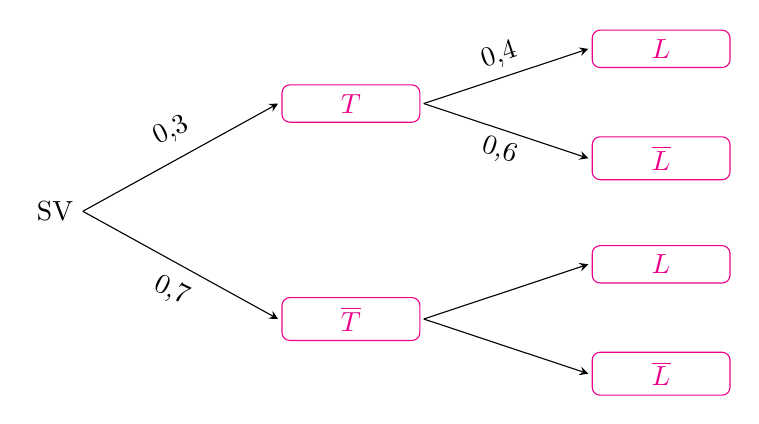
\begin{tikzpicture}
					\def\gocm{20} 
					 \def\gocn{10}
					 \def\r{4}
					\tikzset{s/.style={outer sep=0.5  mm,draw,magenta,rectangle,minimum width=1.75cm,rounded corners=1mm}}
					\path  (0,0) node (O){SV}++(\gocm:\r) node[s](A1){$T$}++(\gocn:\r) node[s](A2){$L$};
					\path (A1)++({-\gocn}:\r)  node[s](a2){$\overline{L}$};
					\path (O)++(-\gocm:\r) node[s](B1){$\overline{T}$}++(\gocn:\r) node[s](B2){$L$}; 
					\path (B1)++({-\gocn}:\r)  node[s](b2){$\overline{L}$};
					 \foreach \x/\y in {
						O/A1,A1/A2, 
						O/B1,B1/B2, 
						A1/a2, 
						B1/b2} 
					\draw[-stealth](\x.east)--(\y.west); 
					 \path (O)--(A1.west) node[pos=0.5,above,sloped]{$\mbox{0{,}3}$}
						(O)--(B1.west) node[pos=0.5,below,sloped]{$\mbox{0{,}7}$} 
						 (B1.east)--(B2.west) node[pos=0.5,above,sloped]{}
						(A1.east)--(A2.west) node[pos=0.5,above,sloped]{$\mbox{0{,}4}$} 
						 (A1.east)--(a2.west) node[pos=0.5,below,sloped]{$\mbox{0{,}6}$}
						(B1.east)--(b2.west) node[pos=0.5,below,sloped]{}; 
				\end{tikzpicture}
		\end{center}
		\begin{itemchoice}
			\itemch Vì xác suất gặp sinh viên thi trượt  cả môn Toán và Tâm Lý là
			$$\mathrm{P} \left(TL\right)=\mathrm{P} \left(T\right)\mathrm{P} \left( L|T  \right)=0{,}3 \cdot 0{,}4=0{,}12.$$
			\itemch Xác suất gặp  sinh viên đậu cả môn Toán và Tâm lý là
			$$\mathrm{P} \left(\overline{T}  \overline{L} \right)=1-\mathrm{P} \left(T\cup L\right)=1-\mathrm{P}\left(T \right)-\mathrm{P}\left(L \right)+\mathrm{P}\left(TL\right)=1-0{,}3-0{,}22+0{,}12=0{,}6.$$
			\itemch Xác suất gặp sinh viên đậu môn Toán, biết rằng sinh viên này trượt môn Tâm lý  là
			$$\mathrm{P} \left(\overline{T} | L \right)=\dfrac{\mathrm{P}  \left(\overline{T}L\right)}{\mathrm{P}\left(L\right)}=\dfrac{\mathrm{P}\left(L\right)-\mathrm{P}\left(TL\right)}{\mathrm{P}\left(L\right)}=\dfrac{0{,}22-0{,}12}{0{,}22}=0{,}45.$$
			\itemch Xác suất gặp sinh viên đậu môn Tâm  lý là
			$$\mathrm{P} \left(\overline{L}\right)=1- \mathrm{P}\left( L \right)= 1-  0{,}22= 0{,}78.$$
		\end{itemchoice}
	} 
\end{ex}

% nguồn: Lop_12_Dai_so_Chuong_6
\begin{ex}%[2D6V2-2]%[ma:8a8d4eb5]
	Hai đội bóng thực hiện các lượt sút luân lưu. Trong loạt sút thứ nhất, đội bóng thứ nhất  thực hiện trước với xác suất thành công là $0{,}8$, đội bóng thứ hai thực hiện sau. Nếu cầu thủ của đội bóng thứ nhất thực hiện thành công quả đá đầu tiên thì cầu thủ của đội bóng thứ hai có xác suất thực hiện thành công là $0{,}7$; nếu đội bóng thứ nhất thực hiện không thành công thì xác suất để đội bóng thứ hai thực hiện thành công là $0{,}9$. Xét các biến cố sau:\\
	Gọi $A$ là biến cố \lq\lq Cầu thủ của  đội bóng thứ nhất thành công\rq\rq. \\
	Gọi $B$ là biến cố \lq\lq Cầu thủ của đội bóng thứ hai  thành công\rq\rq.
	 \choiceTF
		{$\mathrm{P}  \left(B|A\right)=0{,}9$}
		{\True $\mathrm{P}  \left(\overline{B}| A\right)=0{,}3$}
		 {\True $\mathrm{P} \left(AB\right)=0{,}56$}
		{$\mathrm{P} \left(\overline{B}\right)=0{,}16$} 
	\loigiai{ 
		Theo đề bài ta có $\mathrm{P} \left(A\right)=0{,}8$; $\mathrm{P} \left(B|A\right) = 0{,}7$;  $\mathrm{P}\left(B| \overline{A} \right) = 0{,}9$.
		\begin{itemchoice}
			\itemch $\mathrm{P} \left(B|A\right)$ là xác suất cầu thủ của đội bóng thứ hai thành công nếu cầu thủ của đội bóng thứ  nhất thành công. Do đó, $\mathrm{P} \left(B|A\right)=0{,}7$.
			\itemch $\mathrm{P} \left(\overline{B} | A \right)=1-\mathrm{P} \left(B|A\right)=1-0{,}7=0{,}3$. 
			\itemch $\mathrm{P}  \left(AB \right)=\mathrm{P} \left(A\right) \cdot \mathrm{P} \left(B|A\right)=0{,}8\cdot 0{,}7=0{,}56$.
			\itemch $B$ là biến cố “Cầu thủ của đội bóng  thứ hai thực hiện thành công”.\\
			Khi đó, ta  có\\
			$\mathrm{P} \left(B\right)=\mathrm{P}  \left(A\right) \cdot \mathrm{P} \left(B|A\right)+\mathrm{P} \left(\overline{A}\right) \cdot \mathrm{P} \left( B|\overline{A}\right)=0{,}8 \cdot 0{,}7+0{,}2 \cdot 0{,}9=0{,}74$\\
			$\Rightarrow  \mathrm{P} \left(\overline{B}\right)=1-\mathrm{P}\left(B\right)=0{,}26$.
		\end{itemchoice}
	} 
\end{ex}

% nguồn: Lop_12_Dai_so_Chuong_6
\begin{ex}%[2D6V2-2]%[ma:4d032830]
	Một cửa  hàng chỉ bán hai loại điện thoại là Samsung và Iphone. Tỷ lệ khách hàng mua điện thoại Samsung là $75\%$. Trong số các khách hàng mua điện thoại Samsung thì có $60\%$ mua kèm ốp điện thoại. Tỷ lệ khách hàng mua điện thoại Iphone kèm ốp điện thoại trong số những khách hàng mua điện thoại Iphone là $30\%$.
	\choiceTF 
		{\True Xác  suất một khách hàng mua điện thoại Samsung là $0{,}75$}
		{Xác suất  để một khách hàng mua điện thoại Iphone là $0{,}15$}
		{\True Xác suất để một khách hàng mua ốp điện thoại biết rằng khách hàng đó đã mua điện  thoại Samsung là $0{,}6$, xác suất để một khách hàng mua ốp điện thoại biết rằng khách hàng đó đã mua Iphone là $0{,}3$}
		{\True Xác suất một khách hàng  mua điện thoại kèm ốp là $0{,}525$}
	\loigiai{ 
		Gọi $A$ là biến cố \lq\lq một khách hàng mua điện thoại kèm ốp\rq\rq,  $B$ là biến cố \lq\lq một khách hàng mua điện thoại Samsung\rq\rq.
		\begin{itemchoice}
			\itemch $\mathrm{P}  \left(B\right)=75\%=0{,}75$.
			\itemch Xác suất để một khách hàng mua  điện thoại Iphone là $\mathrm{P} \left(\overline{B}\right)=1-0{,}75=0{,}25$.
			\itemch $\mathrm{P} \left( A|B\right)=60\%=0{,}6$; $\mathrm{P} \left( A|\overline{B}\right)=30\%=0{,}3$. 
			\itemch $\mathrm{P} \left(A\right)=\mathrm{P} \left(B\right)\mathrm{P} \left( A|B\right)+\mathrm{P} \left(\overline{B}\right)\mathrm{P} \left( A|\overline{B}\right)$ $=0{,}75\cdot  0{,}6+0{,}25\cdot 0{,}3=0{,}525$.
		\end{itemchoice}
	 }
\end{ex}

% nguồn: Lop_12_Dai_so_Chuong_6
\begin{ex}%[2D6V2-2]%[ma:0e076b7c]
	Có $2$ xạ thủ loại $I$ và $8$ xạ thủ loại $II$, xác  suất bắn trúng đích của các xạ thủ loại $I$ là $0{,}9$ và loại $II$ là $0{,}7$. Khi đó
	 \choiceTF
		{Chọn ngẫu nhiên $1$ xạ thủ bắn và xạ thủ đó bắn một viên đạn. Gọi $A$ là biến cố \lq\lq Viên đạn trúng đích\rq\rq. $B$ là biến cố \lq\lq Xạ thủ loại $I$ bắn\rq\rq. $C$ là biến cố \lq\lq Xạ thủ loại $II$ bắn\rq\rq. Khi đó ta có xác suất để viên  đạn trúng đích được tính theo công thức công thức:
		$\mathrm{P}(A)=\mathrm{P}(B) \cdot  \mathrm{P}(A\mid B)+\mathrm{P}(C)\cdot\mathrm{P}\left(A\mid \overline{C}\right)$}
		{\True Chọn ngẫu nhiên một xạ thủ bắn và xạ thủ đó bắn một viên đạn. Xác suất để viên đạn đó trúng đích là  $0{,}74$}
		{Chọn  ngẫu nhiên ra hai xạ thủ và cả hai xạ thủ đều bắn một viên đạn. Gọi $E$ là biến cố \lq\lq Cả hai viên đạn đều bắn trúng đích\rq\rq\, $E_{i} $ là biến cố chọn được $i$ xạ thủ loại $I$. Khi đó ta có công thức tính xác xuất để cả hai xạ thủ đều bắn trúng là\\
		$\mathrm{P}(E)=\mathrm{P}(E_{0})\cdot\mathrm{P}(E\mid  E_{0})+\mathrm{P}(E_{1})\cdot\mathrm{P}\left(E\mid \overline{E_{1} }\right)+\mathrm{P}(E_{2})\cdot\mathrm{P}\left(E\mid \overline{E_{2} }\right)$}
		{Chọn ngẫu nhiên hai  xạ thủ, mỗi người bắn một viên đạn. Xác suất để cả hai viên đạn đó trúng đích là $0{,}596$}
	\loigiai{ 
		\begin{itemchoice}
			 \itemch Ta có $\mathrm{P}(A)=\mathrm{P}(B) \cdot \mathrm{P}(A\mid B)+\mathrm{P}(C)\cdot \mathrm{P}(A\mid C)$
			\itemch Gọi $A$ là biến cố \lq\lq  Viên đạn trúng đích\rq\rq;\\
			$B$ là biến cố  \lq\lq Xạ thủ loại I bắn\rq\rq;\\
			$C$ là biến cố  \lq\lq Xạ thủ loại II bắn\rq\rq.\\
			Ta có $\mathrm{P}(B)=\dfrac{2}{10} =0{,}2$;  $\mathrm{P}(A\mid B)=0{,}9$; $ \mathrm{P}(C)=\dfrac{8}{10} =0{,}8$; $\mathrm{P}(A\mid C)=0{,}7$.\\
			$B$ và $C$ tạo thành họ đầy đủ các biến cố nên \[\mathrm{P}(A)=\mathrm{P}(B) \cdot  \mathrm{P}(A\mid B)+\mathrm{P}(C)\cdot\mathrm{P}(A\mid C)
			 =0{,}2\cdot0{,}9+0{,}8\cdot0{,}7=0{,}74.\]
			\itemch $E_{i} $ là biến cố  chọn được $i$ xạ thủ loại $I$ nên
			\[\mathrm{P}(E)=\mathrm{P}(E_{0})\cdot\mathrm{P}(E\mid E_{0})+\mathrm{P}(E_{1})\cdot\mathrm{P}(E\mid E_{1})+\mathrm{P}(E_{2})  \cdot \mathrm{P}(E\mid E_{2}).\]
			\itemch Gọi $E$ là biến cố \lq\lq Cả hai viên đạn đều  bắn trúng đích\rq\rq. Ta có
			\begin{itemize}
				\item $\mathrm{P}(E_{0})=  \dfrac{\mathrm{C}_{8}^2}{\mathrm{C}_{10}^2} =\dfrac{28}{45}$; $\mathrm{P}(E\mid E_{0})=0{,}7\cdot0{,}7=0{,}49$;
				\item $\mathrm{P}(E_{1})=\dfrac{\mathrm{C}_{2}^1 \cdot \mathrm{C}_8^1}{\mathrm{C}_{10}^2} =\dfrac{16}{45}$; $\mathrm{P}(E\mid E_{1})=0{,}9\cdot  0{,}7=0{,}63$;
				 \item $\mathrm{P}(E_{2})=\dfrac{\mathrm{C}_{2}^2}{\mathrm{C}_{10}^2} =\dfrac{1}{45} $; $ \mathrm{P}(E\mid E_{2})=0{,}9\cdot 0{,}9=0{,}81$.
			\end{itemize}
			 Vì $E_{0}$, $E_{1} $, $E_{2} $ tạo thành họ đầy đủ các biến cố nên ta có xác suất để cả hai viên đạn đó trúng đích là
			\begin{align*}
				\mathrm{P}(E)=& \mathrm{P}(E_{0})\cdot  \mathrm{P}(E\mid E_{0})+\mathrm{P}(E_{1})\cdot \mathrm{P}(E\mid E_{1})+\mathrm{P}(E_{2})\cdot\mathrm{P}(E\mid E_{2})\\
				 =& \dfrac{28}{45} \cdot 0{,}49+\dfrac{16}{45} \cdot 0{,}63+\dfrac{1}{45} \cdot 0{,}81=0{,}5469.
			\end{align*}
		\end{itemchoice}
	 }
\end{ex}


%%%%%%%%%%%%%%%% TRẢ LỜI NGẮN %%%%%%%%%%%%%%%%

% nguồn: Lop_12_Dai_so_Chuong_6
\begin{bt}%[2D6H2-2]%[ma:ad51b5fe]
	Một lớp có $16$ học sinh nữ, còn lại là học sinh nam. Trong giờ giáo dục thể chất thầy giáo khảo sát kết quả rèn luyện  thể lực của học sinh bằng cách bốc thăm trong danh sách lớp để chọn hai bạn chạy tiếp sức. Biết xác suất để chọn được hai bạn tham gia khảo sát đều là nữ bằng $\dfrac{15}{62}$. Hỏi lớp đó có bao nhiêu học sinh?
	 \shortans{32}
	 \loigiai{
		Gọi $A$ là biến cố  \lq\lq Lần thứ nhất chọn được bạn nữ\rq\rq.\\
		Gọi $B$ là biến cố \lq\lq Lần thứ hai  chọn được bạn nữ\rq\rq.\\
		Gọi $C$ là biến cố \lq\lq Chọn được hai bạn tham gia khảo sát đều là nữ\rq\rq.\\ 
		Theo đề bài ta có  $C=AB\Rightarrow \mathrm{P}\left(C\right)=\mathrm{P}\left(AB\right)=\dfrac{15}{62} $.\\
		Gọi số học sinh của lớp là  $x$, $x \in \mathbb{N}$, $x>16$.\\
		Theo đề  bài ta có $ \mathrm{P}\left(A\right)=\dfrac{16}{x}$, $\mathrm{P}\left(B\mid A\right)=\dfrac{15}{x-1}$.\\
		Do $ \mathrm{P}\left(AB\right) = \mathrm{P}\left(BA\right) = \mathrm{P}\left(B\mid A\right)\cdot \mathrm{P}\left(A\right) \Leftrightarrow  \dfrac{15}{62} = \dfrac{16}{x} \cdot \dfrac{15}{x-1} \Leftrightarrow x^2 - x - 992 = 0 \Leftrightarrow \hoac{&x=32\\&x=-31.}$\\
	Vậy số học sinh của lớp là $32$ học sinh.} 
\end{bt}

% nguồn: Lop_12_Dai_so_Chuong_6
\begin{bt}%[2D6H2-2]%[ma:5beb9d48]
	Một loại xét nghiệm nhanh SARS-CoV-2 cho kết quả dương tính với tỉ  lệ $76{,}2\%$ các ca thực sự nhiễm virus và kết quả âm tính với tỉ lệ $99{,}1\%$ các ca thực sự không nhiễm virus \textit{(nguồn: https://tapchiyhocvietnam.vn/index.php/vmj/article/view/2124/1921)}.
	Giả sử tỉ  lệ người nhiễm virus SARS-CoV-2 trong một cộng đồng là $1\%$. Hãy tính xác suất người làm xét nghiệm có kết quả dương tính (kết quả làm tròn đến hàng phần trăm).
	 \shortans{0,02}
	\loigiai{ 
		Gọi $A$ là biến cố \lq\lq  Người làm xét nghiệm có kết quả dương tính\rq\rq.\\
		$B$ là biến cố \lq\lq  Người làm xét nghiệm thực sự nhiễm virus\rq\rq.\\
		 Do xét nghiệm cho kết quả dương tính với tỉ lệ $76{,}2\%$ các ca thực sự nhiễm virus nên ta có $\mathrm{P}(A\mid B) = 0{,}762$.\\
		Do xét nghiệm cho kết quả âm tính với tỉ lệ $99{,}1\%$ các ca thực sự không nhiễm virus nên ta  có $\mathrm{P}(\overline{A}\mid\overline{B}) = 0{,}991$.\\
		Suy ra $\mathrm{P}\left(A\mid\overline{B}\right)  = 1-0{,}991 = 0{,}009$.\\
		Do tỉ lệ người  nhiễm virus trong cộng đồng là $1\%$ nên ta có $\mathrm{P}(B) = 0{,}01$ và $\mathrm{P}(\overline{B}) = 0{,}99$.\\
		Áp dụng công thức xác suất toàn phần, ta có xác suất người làm  xét nghiệm có kết quả dương tính là
		\begin{eqnarray*}
			\mathrm{P}(A) &=& \mathrm{P}(B)\cdot\mathrm{P}(A\mid B) + \mathrm{P}\left(\overline{B}\right)\cdot\mathrm{P}\left(A\mid \overline{B}\right)\\ 
			&=& 0{,}01 \cdot 0{,}762  + 0{,}99 \cdot 0{,}009\\
			 &=& 0{,}01653 \approx 0{,}02.
		\end{eqnarray*}
	 }
\end{bt}

% nguồn: Lop_12_Dai_so_Chuong_6
\begin{bt}%[2D6H2-2]%[ma:e8e09122]
	Giả sử tỷ lệ người dân của tỉnh M nghiện thuốc lá là $20\%$, tỷ lệ người dân bị bệnh phổi là $26\%$, trong số người bị bệnh phổi thì tỷ lệ nghiện thuốc lá là $70\%$. Tính xác suất người đó nghiện thuốc  lá khi biết bị bệnh phổi (làm tròn kết quả đến hàng phần trăm).
	 \shortans{0,54}
	 \loigiai{
		Gọi $A$ là biến cố \lq\lq người nghiện thuốc lá\rq\rq\ $\Rightarrow  \mathrm{P}(A)=0{,}2$.\\
		Gọi $B$ là biến cố \lq\lq người bị  bệnh phổi\rq\rq\ $\Rightarrow \mathrm{P}(B)=0{,}26$.\\
		Trong số người bị bệnh phổi,  tỷ lệ nghiện thuốc lá là $70\%$ $\Rightarrow \mathrm{P}(B \mid A)=0{,}7$.\\
	Khi đó $\mathrm{P}(A \mid B)=\dfrac{\mathrm{P}(A)\mathrm{P}(B  \mid A)}{\mathrm{P}(B)}=\dfrac{0{,}2\cdot 0{,}7}{0{,}26}=\dfrac{7}{13}\approx0{,}54$. }
\end{bt}

% nguồn: Lop_12_Dai_so_Chuong_6
\begin{bt}%[2D6H2-2]%[ma:47ed1c48]
	Điều tra người dân trong một tỉnh, người ta thấy tỉ lệ nghiện rượu, bia là $30\%$. Tỉ lệ người mắc bệnh  về gan trong số những người nghiện rượu, bia là $60\%$ và tỉ lệ người mắc bệnh về gan trong số những người không nghiện rượu, bia là $10\%$. Chọn ngẫu nhiên một người dân của tỉnh đó. Tính xác suất để người đó mắc bệnh về gan? (Viết kết quả dưới dạng thập phân)
	\shortans{0,25} 
	\loigiai{Gọi  $A$ là biến cố người được chọn nghiện rượu, bia.\\
		Gọi $G$ là biến cố người được  chọn mắc bệnh về gan.\\
		Theo đề bài, ta có $\mathrm{P}(A) = 0{,}3$. Suy ra $\mathrm{P}(\overline{A}) = 1 - \mathrm{P}(A)  = 1 - 0{,}3 = 0{,}7$.\\
		Tỉ lệ người mắc  bệnh về gan trong số những người nghiện rượu, bia là $\mathrm{P}(G \mid A) = 0{,}6$.\\
		Tỉ lệ người mắc bệnh về gan trong số những người không nghiện rượu, bia là $\mathrm{P}(G \mid \overline{A})  = 0{,}1$.\\
		Áp dụng công thức xác suất toàn phần,  xác suất để người đó mắc bệnh về gan là\\
		$\mathrm{P}(G) = \mathrm{P}(A) \cdot  \mathrm{P}(G \mid A) + \mathrm{P}(\overline{A}) \cdot \mathrm{P}(G \mid \overline{A})$.\\
	$\mathrm{P}(G) = 0{,}3 \cdot 0{,}6 + 0{,}7\cdot 0{,}1  = 0{,}18 + 0{,}07 = 0{,}25$.\\}
\end{bt}

% nguồn: Lop_12_Dai_so_Chuong_6
\begin{bt}%[2D6H2-2]%[ma:7982cac4]
	Một cơ sở sản xuất sữa giả mua các thùng sữa thật giống nhau ($48$ hộp / thùng), rồi thay thế một số hộp sữa thật thành các hộp sữa giả nhằm thu lợi bất chính.  Trong quá trình sản xuất, cơ sở phân ra làm hai loại: Loại I để lẫn mỗi thùng 5 hộp sữa giả và loại II để lẫn mỗi thùng $3$ hộp sữa giả. Biết rằng số thùng sữa loại I gấp $1{,}5$ lần số thùng sữa loại II. Chọn ngẫu nhiên một thùng sữa từ cơ sở sản xuất và từ thùng đó lấy ngẫu nhiên $10$ hộp. Tính xác suất để trong $10$ hộp lấy ra có đúng $2$ hộp sữa là giả (làm tròn kết quả đến hàng phần trăm).
	\shortans{0,17} 
	\loigiai{ 
		Gọi biến cố $A$ là biến cố  chọn được \lq \lq Thùng sữa loại I\rq \rq.\\
		Biến cố $\overline{A}$ là biến cố chọn được \lq \lq Thùng  sữa loại II\rq \rq.\\
		Nếu số thùng sữa loại II là $x$ thùng ($x\in\mathbb{N}$) thì số thùng  sữa loại I là $1{,}5x$ thùng.\\
		Khi đó  $\mathrm{P}\left(A\right)=\dfrac{1{,}5x}{1{,}5x+x}=\dfrac{3}{5}$; $\mathrm{P}(\overline{A})=1-\mathrm{P}\left(A\right)=\dfrac{2}{5}$.\\
		Gọi biến  cố $B$ là biến cố chọn được \lq \lq10 hộp lấy ra có đúng 2 hộp sữa giả\rq \rq.\\
		Ta có $\mathrm{P}(B|A)=\dfrac{C_5^2C_{43}^8}{C_{48}^{10}}$  và $\mathrm{P}(B|\overline{A})=\dfrac{C_3^2C_{45}^8}{C_{48}^{10}}$.\\
		Vậy  $\mathrm{P}\left(B\right)=\mathrm{P}\left(A\right)\cdot \mathrm{P}(B|A)+\mathrm{P}(\overline{A})\cdot \mathrm{P}(B|\overline{A})=\dfrac{3}{5}\dfrac{C_5^2C_{43}^8}{C_{48}^{10}}+\dfrac{2}{5}\dfrac{C_3^2C_{45}^8}{C_{48}^{10}}=\dfrac{2052}{11891}\approx 0{,}17$.
	 }
\end{bt}

% nguồn: Lop_12_Dai_so_Chuong_6
\begin{bt}%[2D6H2-2]%[ma:baaa22af]
	Một hộp có $80$ viên bi, trong đó có $50$ viên bi màu đỏ và $30$ viên bi màu vàng; các viên bi có kích  thước và khối lượng như nhau. Sau khi kiểm tra, người ta thấy có $90\%$ số viên bi màu đỏ được đánh số và $50\%$ số viên bi màu vàng được đánh số, những viên bi còn lại không đánh số. Lấy ra ngẫu nhiên một viên bi trong hộp. Tính xác suất để viên bi được lấy ra có đánh số (làm tròn kết quả đến hàng phần trăm).
	\shortans{0,75} 
	 \loigiai{
		Gọi $A$ là  biến cố \lq\lq Viên bi được lấy ra có đánh số\rq\rq.\\
		Gọi $B$ là biến cố \lq\lq Viên bi được lấy ra có màu đỏ\rq\rq, suy ra $\overline{B}$ là  biến cố \lq\lq Viên bi được lấy ra có màu vàng\rq\rq.\\
		Khi  đó, ta có
		\begin{itemize}
			\item $\mathrm{P}(B) = \dfrac{50}{80} = \dfrac{5}{8}$; \quad $\mathrm{P}\big(\overline{B}\big)  = \dfrac{30}{80} = \dfrac{3}{8}$.
			\item $\mathrm{P}\big(A \mid B\big) = 90\% = \dfrac{9}{10}$; \quad $\mathrm{P}\big(A \mid \overline{B}\big) = 50\%  = \dfrac{1}{2}$.
		\end{itemize}
		Áp dụng công thức xác suất toàn phần, ta  có
		 \[
		 \mathrm{P}(A)
		=  \mathrm{P}(B) \cdot \mathrm{P}\big(A \mid B\big)
		+ \mathrm{P}\big(\overline{B}\big) \cdot \mathrm{P}\big(A \mid \overline{B}\big) 
		= \dfrac{5}{8} \cdot  \dfrac{9}{10}
		+ \dfrac{3}{8} \cdot \dfrac{1}{2} 
		= \dfrac{3}{4} = 0{,}75. 
		\] 
	 }
\end{bt}

% nguồn: Lop_12_Dai_so_Chuong_6
\begin{bt}%[2D6H2-2]%[ma:8492cf33]
	Một kho hàng do hai nhà máy sản xuất. Biết tỉ lệ sản phẩm đóng góp của nhà máy một bằng $\dfrac{1}{3}$ sản phẩm đóng góp của nhà máy hai và tỉ lệ phế phẩm do nhà máy một, nhà máy  hai sản xuất lần lượt là $0{,}1\%$ và $0{,}2\%$. Chọn ngẫu nhiên một sản phẩm thì thấy nó là phế phẩm. Biết xác suất để phế phẩm đó do nhà máy hai sản xuất là $\dfrac{a}{b}$. Tính giá trị biểu thức $T=a+2b$.
	\shortans{20} 
	 \loigiai{
		Gọi $A$ là biến  cố \lq\lq Sản phẩm được chọn là phế phẩm\rq\rq,~
		$B$ là biến cố \lq\lq Sản phẩm được chọn  thuộc nhà máy một\rq\rq.\\
		Khi đó $\overline{B}$ là biến cố \lq\lq Sản  phẩm được chọn thuộc nhà máy hai\rq\rq.\\
		 Ta có
		\begin{itemize}
			\item  $\mathrm{P}(B)=25\%=0{,}25$;
			\item $\mathrm{P}(\overline{B})=75\%=0{,}75$; 
			\item $\mathrm{P}(A\mid B)=0{,}1\%=0{,}001$; 
			\item  $\mathrm{P}\left(A\mid\overline{B}\right)=0{,}2\%=0{,}002$.
		\end{itemize}
		Áp dụng công thức  xác suất toàn phần, ta có xác suất chọn được phế phẩm là
		\begin{eqnarray*}
			 \mathrm{P}(A) &=& \mathrm{P}(B)\cdot \mathrm{P}(A\mid B)+\mathrm{P}\left(\overline{B}\right)\cdot \mathrm{P}\left(A\mid\overline{B}\right)\\
			&=& 0{,}25\cdot 0{,}001+0{,}75\cdot  0{,}002 = \dfrac{7}{4000}.
		\end{eqnarray*}
		Áp dụng công thức Bayes,  ta có
		\[\mathrm{P}(\overline{B}\mid A) = \dfrac{\mathrm{P}\left(\overline{B}\right)\cdot \mathrm{P}\left(A\mid\overline{B}\right)}{\mathrm{P}(A)} = \dfrac{0{,}75\cdot 0{,}002}{\dfrac{7}{4000}}  = \dfrac{6}{7}.\]
		Khi đó xác suất để phế phẩm đó do  nhà máy hai sản xuất là $\dfrac{6}{7}$.\\
		Suy  ra
		 \[\heva{& a=6 \\ & b=7} \Rightarrow T = 6+2\cdot 7 = 20.\]
	 }
\end{bt}

% nguồn: Lop_12_Dai_so_Chuong_6
\begin{bt}%[2D6H2-2]%[ma:4922602b]
	Có hai lô sản phẩm gồm các loại sản phẩm tốt và xấu. Lô $1$ có $50$ sản phẩm trong đó có $20$ sản phẩm xấu, lô $2$ có $40$ sản phẩm trong đó có $15$ sản phẩm xấu. Lấy ngẫu nhiên một lô và từ đó lấy ra một sản phẩm. Tìm xác suất để sản phẩm lấy ra là sản phẩm tốt (kết quả làm tròn đến hàng  phần trăm).
	\shortans{0,61} 
	 \loigiai{
		Gọi $B_1$ là biến cố  \lq\lq Lô được chọn là lô sản phẩm $1$\rq\rq.\\
		$B_2$ là biến cố \lq\lq Lô được  chọn là lô sản phẩm $2$\rq\rq.\\
		$A$ là biến cố \lq\lq sản phẩm lấy ra là sản phẩm  tốt\rq\rq.\\
		Ta  có $\mathrm{P}(B_1) = \mathrm{P}(B_2) = \dfrac{1}{2}$; $\mathrm{P}(A\mid B_1) = \dfrac{30}{50}$; $\mathrm{P}(A\mid B_2) = \dfrac{25}{45}$.\\
		Theo công thức xác suất toàn  phần, ta có
		\[\mathrm{P}(A) = \mathrm{P}(B_1)\cdot\mathrm{P}(A\mid B_1) + \mathrm{P}(B_2)\cdot \mathrm{P}(A\mid B_2) = \dfrac{1}{2}\cdot\dfrac{30}{50} + \dfrac{1}{2}\cdot\dfrac{25}{40}  = 0{,}6125.\]
		Vậy xác suất lấy ra sản phẩm tốt là  $0{,}61$.
	 }
\end{bt}

% nguồn: Lop_12_Dai_so_Chuong_6
\begin{bt}%[2D6H2-2]%[ma:4fc9dc56]
	Một cửa hàng bán giày có hai loại  giày thể thao loại I và loại II. Tỉ lệ số lượng giày mỗi loại trong kho như sau: loại I chiếm $60\%$, loại II chiếm $40\%$. Tỉ lệ giày loại I bị lỗi là $1\%$ và tỉ lệ giày loại II bị lỗi là $3\%$. Một khách hàng đến cửa hàng và chọn mua ngẫu nhiên một đôi giày thể thao. Xác suất để đôi giày mà khách hàng mua bị lỗi là $x\%$. Tính giá trị của $x$ (kết quả được ghi chính xác dưới dạng số thập phân).
	\shortans{1{,8}}%CẦN  KIỂM TRA ĐÁP ÁN
	 \loigiai{
		Gọi $A$ là biến cố: \lq\lq đôi giày mà khách hàng mua là giày  loại I\rq\rq; $B$ là biến cố: \lq\lq đôi giày mà khách hàng mua bị lỗi\rq\rq.\\
		Ta  có $\mathrm{P}(A)=0{,}6$, $\mathrm{P}(\overline{A})=1-0{,}6=0{,}4$.\\
		 $\mathrm{P}(B| A)=0{,}01$, $\mathrm{P}(B|\overline{A})=0{,}03$.\\
		Xác suất để đôi giày mà  khách hàng mua bị lỗi là
		$$\mathrm{P}(B)=\mathrm{P}(B| A)\cdot \mathrm{P}(A)+\mathrm{P}(B| \overline{A})\cdot \mathrm{P}(\overline{A})=0{,}01\cdot  0{,}6+0{,}03\cdot 0{,}4=0{,}018=1{,}8\%.$$
	} 
\end{bt}

% nguồn: Lop_12_Dai_so_Chuong_6
\begin{bt}%[2D6H2-2]%[ma:176f7440]
	Một lô linh kiện có chứa $40\%$ linh kiện do nhà máy I sản xuất và $60\%$ linh kiện do nhà máy II sản xuất. Biết tỉ lệ phế phẩm của nhà máy  I, II lần lượt là $3\%$, $4\%$. Một khách hàng lấy ngẫu nhiên một linh kiện từ lô hàng đó. Tính xác suất để linh kiện được lấy ra là linh kiện tốt (làm tròn kết quả đến hàng phần trăm).
	 \shortans{0,96}
	 \loigiai{
		Gọi $A$ là biến cố \lq\lq Linh kiện được lấy  ra là linh kiện tốt\rq\rq.\\
		Gọi $B$ là biến cố \lq\lq Linh kiện được lấy ra do nhà máy I  sản xuất\rq\rq, suy ra $\overline{B}$ là biến cố \lq\lq Linh kiện được lấy ra do nhà máy II sản xuất\rq\rq.\\
		Khi đó  ta có
		\begin{itemize}
			\item $\mathrm{P}(B) = 40\%  = \dfrac{2}{5}$; \quad $\mathrm{P}\big(\overline{B}\big) = 60\% = \dfrac{3}{5}$.
			\item $\mathrm{P}\big(A \mid B\big) = 100\% -  3\% = 97\% = \dfrac{97}{100}$; \quad $\mathrm{P}\big(A \mid \overline{B}\big) = 100\% - 4\% = 96\% = \dfrac{96}{100} = \dfrac{24}{25}$.
		\end{itemize}
		Áp dụng công thức xác  suất toàn phần, ta có
		 \[
		\mathrm{P}(A) = \mathrm{P}(B) \cdot \mathrm{P}\big(A \mid B\big) + \mathrm{P}\big(\overline{B}\big) \cdot \mathrm{P}\big(A \mid  \overline{B}\big)
		= \dfrac{2}{5} \cdot \dfrac{97}{100}  + \dfrac{3}{5} \cdot \dfrac{24}{25}
		= \dfrac{241}{250}  \approx 0{,}96.
		\] 
	 }
\end{bt}

% nguồn: Lop_12_Dai_so_Chuong_6
\begin{bt}%[2D6V2-2]%[ma:1b2fb6af]
	Xác suất bé An được mẹ dẫn theo khi đi mua sắm là $\dfrac{2}{5}$. Khi bé An được đi theo mẹ thì $70\%$ bé sẽ được mua đồ chơi.  Khi bé không đi theo mẹ, có thể mẹ vẫn mua đồ chơi cho bé. Xác suất bé được đi theo mẹ biết rằng bé được mẹ mua cho đồ chơi là $\dfrac{14}{23}$. Khi bé không đi theo mẹ, xác suất bé được mẹ mua cho đồ chơi là bao nhiêu? \shortans{0,3}
	 \loigiai{
		Gọi  $A$ là biến cố \lq\lq Bé An được mẹ dẫn theo khi đi mua sắm\rq\rq.\\
		Gọi $B$ là biến  cố \lq\lq Bé An được mẹ mua đồ chơi\rq\rq.\\
		Ta  cần tính $\mathrm{P}\left(B\mid \overline{A}\right)$.\\
		Theo đề bài, ta  có
		\begin{itemize}
			 \item $\mathrm{P}(A)=\dfrac{2}{5}$;
			\item $\mathrm{P}\left(\overline{A}\right)=\dfrac{3}{5}$; 
			\item  $\mathrm{P}(B\mid A)=70\%=\dfrac{7}{10}$;
			\item $\mathrm{P}(A\mid B)=\dfrac{14}{23}$. 
		\end{itemize}
		 Ta có
		\[\mathrm{P}(B)\cdot \mathrm{P}(A\mid  B)=\mathrm{P}(A)\cdot \mathrm{P}(B\mid A)\Rightarrow \mathrm{P}(B)=\dfrac{2}{5}\cdot\dfrac{7}{10}\cdot\dfrac{23}{14}=\dfrac{23}{50}.\]
		Mặt khác, theo công thức xác suất toàn phần, ta  có
		\allowdisplaybreaks 
		\begin{eqnarray*}
			&\mathrm{P}(B)&=\mathrm{P}(A)\cdot \mathrm{P}(B\mid  A)+\mathrm{P}\left(\overline{A}\right)\cdot \mathrm{P}\left(B\mid \overline{A}\right)\\
			&\Leftrightarrow&\dfrac{23}{50}=\dfrac{2}{5}\cdot\dfrac{7}{10}+\dfrac{3}{5}\cdot  \mathrm{P}\left(B\mid \overline{A}\right)\\
			&\Leftrightarrow& \mathrm{P}\left(B\mid  \overline{A}\right)=\dfrac{3}{10}=0{,}3.
		\end{eqnarray*}
	 }
\end{bt}

% nguồn: Lop_12_Dai_so_Chuong_6
\begin{bt}%[2D6V2-2]%[ma:e11d56de]
	Một nhà máy  sản xuất bóng đèn có tỉ lệ bóng đèn đạt tiêu chuẩn là $80\%$. Trước khi xuất ra thị trường, mỗi bóng đèn đều được kiểm tra chất lượng. Vì sự kiểm tra không thể tuyệt đối hoàn hảo nên tỉ lệ công nhận một bóng đèn đạt tiêu chuẩn là $0{,}9$ và tỉ lệ loại bỏ một bóng hỏng là $0{,}95$. Hãy tính tỉ lệ bóng đạt tiêu chuẩn sau khi qua khâu kiểm tra chất lượng (kết quả để dưới dạng số thập phân và làm tròn đến hàng phần trăm).
	 \shortans{0,73}
	 \loigiai{
		 Gọi $A$ là biến cố \lq\lq bóng đạt chuẩn sau khi qua kiểm tra chất lượng\rq\rq .\\
		Gọi $B$ là biến cố \lq\lq sản phẩm đạt  tiêu chuẩn\rq\rq .\\
		Theo  bài ra ta có $\mathrm{P} \left(B\right)=0{,}8$; $ \mathrm{P} \left(\overline{B}\right)=1-0{,}8=0{,}2$.\\
		Do tỉ lệ công nhận một bóng đèn  đạt tiêu chuẩn là $0{,}9$ nên $ \mathrm{P} \left(A|B\right)=0{,}9$.\\
		Tỉ  lệ loại bỏ một bóng hỏng là $0{,}95$ nên $ \mathrm{P} \left(A|\overline{B}\right)=1-0{,}95=0{,}05$.\\
		Theo công thức xác suất  toàn phần ta có
		\[\mathrm{P} \left(A\right)=\mathrm{P} \left(B\right) \cdot \mathrm{P} \left(A|B\right)+\mathrm{P}\left(\overline{B}\right) \cdot \mathrm{P}  \left(A|\overline{B}\right)=0{,}8 \cdot 0{,}9+0{,}2 \cdot 0{,}05=0{,}73.\]
	} 
\end{bt}

% nguồn: Lop_12_Dai_so_Chuong_6
\begin{bt}%[2D6V2-2]%[ma:efc99e2a]
	Một hộp đựng $50$ bút bi xanh và $50$ bút bi đỏ, các bút bi có cùng kích  thước và khối lượng như nhau. Sau khi thống kê, người ta thấy: có $80\%$ số bút bi xanh có dán tem T/L và $70\%$ số bút bi đỏ có dán tem T/L, những bút bi còn lại không dán tem T/L. Lấy ngẫu nhiên một bút bi trong hộp. Tính xác suất để bút bi được lấy ra có dán tem T/L.
	\shortans{0,75} 
	\loigiai{Gọi $A$ là biến  cố "Bút bi được chọn có dán tem T/L;
	$B$ là biến cố "Bút bi được chọn  có màu xanh".\\
	Khi đó $\overline{B}$ là biến cố "Bút bi được chọn có màu  đỏ".\\
	Ta có $\mathrm{P}\left(B\right)=0{,}5\Rightarrow \mathrm{P}\left(\overline{B}\right)=0{,}5$; $\mathrm{P}\left(A\mid B\right)=0{,}8\Rightarrow \mathrm{P}\left(A\mid  \overline{B}\right)=0{,}7$.\\
	Áp dụng công thức xác suất toàn phần, ta có xác suất lấy được bút bi  có dán tem T/L là
	 \[\mathrm{P}\left(A\right)=\mathrm{P}\left(B\right)\cdot\mathrm{P}\left(A\mid B\right)+\mathrm{P}\left(\overline{B}\right)\cdot\mathrm{P}\left(A\mid \overline{B}\right)=0{,}5\cdot0{,}8+0{,}5\cdot0{,}7=0{,}75.\]}
\end{bt}

% nguồn: Lop_12_Dai_so_Chuong_6
\begin{bt}%[2D6V2-2]%[ma:be7bf175]
	Ông An hàng ngày đi làm bằng xe máy hoặc xe buýt.  Nếu hôm nay ông đi làm bằng xe buýt thì xác suất để hôm sau ông đi làm bằng xe máy là $0{,}4$. Nếu hôm nay ông đi làm bằng xe máy thì xác suất để hôm sau ông đi làm bằng xe buýt là $0{,}7$. Xét một tuần mà thứ hai ông An đi làm bằng xe buýt. Tính xác suất đề thứ tư trong tuần đó ông An đi làm bằng xe máy.
	\shortans{0,36} 
	\loigiai{Gọi $A$ là  biến cố "Thứ ba ông An đi làm bằng xe máy"; $B$ là biến cố "Thứ tư ông An đi làm bằng xe máy".\\
		Khi  đó $\mathrm{P}\left(\overline{B}\mid A\right)=0{,}7$ và $\mathrm{P}\left(B\mid \overline{A}\right)=0{,}4$.\\
		Vì thứ hai, ông An đi làm bằng  xe buýt nên xác suất để thứ Ba (hôm sau), ông đi làm bằng xe máy là $0{,}4$.\\
		 Nên $\mathrm{P}\left(A\right)=0{,}4$.\\
		Suy ra $\mathrm{P}\left(\overline{A}\right)=1-0{,}4=0{,}6$.\\ 
		Theo công thức xác suất toàn phần, ta  có
		\begin{eqnarray*}
			\mathrm{P}(B)&=&\mathrm{P}(A)\cdot \mathrm{P}(B\mid  A)+\mathrm{P}\left(\overline{A}\right)\cdot \mathrm{P}(B\mid \overline{A})\\
			&=&\mathrm{P}(A)\cdot \left(1-\mathrm{P}(\overline{B}\mid A)\right)+\mathrm{P}\left(\overline{A}\right)\cdot\mathrm{P}\left(B\mid \overline{A}\right)  \\
			&=&0{,}4\cdot (1-0{,7})+0{,}6\cdot  0{,}4=0{,}36.
		\end{eqnarray*}
	 }
\end{bt}

% nguồn: Lop_12_Dai_so_Chuong_6
\begin{bt}%[2D6V2-2]%[ma:fbd68534]
	Bạn An phải thực hiện hai thí nghiệm liên tiếp. Thí nghiệm thứ nhất có xác suất thành công là $0{,}7$. Nếu thí nghiệm thứ nhất thành công thì xác suất thành công của thí nghiệm thứ hai là $0{,}9$. Tính xác suất để thí nghiệm thứ nhất thành  công và thí nghiệm thứ hai không thành công.
	 \shortans{0,07}
	\loigiai{ 
		Gọi $A$ là biến cố \lq\lq  Thí nghiệm thứ nhất thành công\rq\rq. Ta có $\mathrm{P}(A)=0{,}7$.\\
		Gọi $B$ là biến  cố \lq\lq Thí nghiệm thứ hai thành công\rq\rq.\\
		Xác suất thí nghiệm thứ hai thành công nếu thí nghiệm thứ nhất đã thành công là \[\mathrm{P}(B\mid  A)=0{,}9.\]
		Xác suất để thí nghiệm thứ hai không thành công, với điều kiện thí  nghiệm thứ nhất đã thành công là
		\[\mathrm{P}(\overline{B}|A)=1-\mathrm{P}(B\mid A)=1-0{,}9=0{,}1. \] 
		Vậy, xác suất để thí nghiệm  thứ nhất thành công và thí nghiệm thứ hai không thành công là
		\[\mathrm{P}(A \cap \overline{B})=\mathrm{P}(A) \cdot \mathrm{P}(\overline{B}|A)=0{,}7  \cdot 0{,}1=0{,}07. \]
	 }
\end{bt}

% nguồn: Lop_12_Dai_so_Chuong_6
\begin{bt}%[2D6V2-2]%[ma:76f89bbb]
	Có hai hộp đựng bi. Hộp thứ nhất có $ 2$ viên bi màu xanh, $ 5$ viên bi màu đỏ, hộp thứ hai có $ 3$ viên bi màu xanh, $ 2$ viên bi màu đỏ. Chọn ngẫu nhiên một hộp, từ đó lấy ngẫu nhiên ra một viên bi. Tính xác suất lấy được viên bi màu đỏ (kết quả làm tròn đến hàng  phần trăm).
	\shortans{0,56} 
	 \loigiai{
		Gọi $  A$ là biến cố: \lq\lq Lấy được viên bi màu đỏ\rq\rq.\\
		Gọi $H_i$ là biến cố: \lq\lq Lấy được  hộp thứ $i$\rq\rq , $\left(i=1; 2\right)$.\\
		Nhận xét: $ \mathrm{P} \left(H_1\right)=\mathrm{P} \left(H_2\right)=\dfrac{1}{2}$ nên $ \mathrm{P}\left(A|H_1\right)=\dfrac{5}{7}$; $\mathrm{P}\left(A|H_2\right)=\dfrac{2}{5}$.\\ 
		Áp dụng xác  suất toàn phần ta có xác suất lấy được viên bi màu đỏ là
		$$ \mathrm{P} \left(A\right)=\mathrm{P} \left(H_1\right) \cdot \mathrm{P} \left(A|H_1\right)+\mathrm{P}  \left(H_2\right) \cdot \mathrm{P} \left(A|H_2\right)=\dfrac{1}{2} \cdot \dfrac{5}{7}+\dfrac{1}{2} \cdot \dfrac{2}{5}=\dfrac{39}{70} \approx 0{,}56.$$
	} 
\end{bt}

% nguồn: Lop_12_Dai_so_Chuong_6
\begin{bt}%[2D6V2-2]%[ma:4633e563]
	Một nhà máy sản xuất bóng đèn có tỉ lệ bóng đạt chuẩn $80\%$. Mỗi bóng đèn đều được kiểm tra, biết rằng tỉ lệ công nhận đúng bóng đạt là $0{,}9$, và tỉ lệ loại bỏ đúng bóng hỏng là $0{,}95$. Hãy tính tỉ lệ bóng được công nhận đạt sau  kiểm tra.
	\shortans{0,73} 
	\loigiai{ 
		Gọi $A$ là biến cố \lq\lq bóng đèn được công nhận đạt\rq\rq;  $B$ là biến cố \lq\lq bóng đèn thật sự đạt chuẩn\rq\rq.\\
		Khi  đó, ta có
		\[\mathrm \mathrm{P}(B)=0{,}8; \quad \mathrm \mathrm{P}(\overline{B})=0{,}2;  \quad
		\mathrm{P}(A\mid B)=0{,}9; \quad \mathrm{P}(A\mid \overline{B})=1-0{,}95=0{,}05.\] 
		Theo công thức xác suất toàn phần,  ta có
		\[ 
		\mathrm  \mathrm{P}(A)=0{,}8\cdot0{,}9+0{,}2\cdot0{,}05=0{,}73.
		 \]
		Vậy tỉ lệ cần tìm là  $0{,}73$.
	} 
\end{bt}

% nguồn: Lop_12_Dai_so_Chuong_6
\begin{bt}%[2D6V2-2]%[ma:6a3f47c4]
	Một hộp chứa $10$ viên bi, trong đó có $6$ viên bi màu đỏ và $4$ viên bi màu xanh. Hai bạn An và Bình lần lượt lấy ra một viên bi từ hộp một cách ngẫu nhiên, bi được lấy ra không bỏ lại hộp. Tính xác suất bạn Bình lấy được một viên bi xanh (làm tròn kết quả đến hàng phần chục). 
	\shortans{0,4} 
	 \loigiai{
		Xét  hai biến cố \\
		$A$: \lq\lq Bạn Bình lấy được một viên  bi xanh\rq\rq;\\
		$B$:  \lq\lq Bạn An lấy được một viên bi xanh\rq\rq.\\
		Khi đó,  ta có $$ \mathrm{P}\left(B\right)=\dfrac{4}{10}=\dfrac{2}{5};\,
		\mathrm{P}  \left(\overline{B}\right)=1-\mathrm{P} \left(B\right)=\dfrac{3}{5};\,
		\mathrm{P}  \left(A|B\right)=\dfrac{3}{9}=\dfrac{1}{3};\,
		\mathrm{P}  \left(A|\overline{B}\right)=\dfrac{4}{9}.$$
		Áp dụng công thức toàn  phần, ta có
	$$  \mathrm{P} \left(A \right)=\mathrm{P} \left(B\right) \cdot \mathrm{P} \left(A|B\right)+\mathrm{P} \left(\overline{B}\right) \cdot \mathrm{P} \left(A|\overline{B}\right)=\dfrac{2}{5} \cdot \dfrac{1}{3}+\dfrac{3}{5} \cdot \dfrac{4}{9}=\dfrac{2}{5} = 0{,}4.$$}
\end{bt}

% nguồn: Lop_12_Dai_so_Chuong_6
\begin{bt}%[2D6V2-2]%[ma:22943515]
	Tại một địa phương có $ 500$ người cao tuổi, bao gồm $260$ nam và $240$ nữ. Trong đó nhóm người cao tuổi nam và nữ lần lượt có $40\%$ và $55\%$ bị bệnh tiểu đường. Chọn ngẫu nhiên một người. Xác suất để chọn được một người không bị bệnh tiểu đường là  bao nhiêu? (làm tròn kết quả đến chữ số hàng phần trăm).
	\shortans{0,53} 
	\loigiai{ 
		 Xét các biến cố:\\
		$ A$: \lq\lq Chọn được  người không bị tiểu đường\rq\rq;\\
		$ B$: \lq\lq Chọn được người cao tuổi là  nam\rq\rq;\\
		$\overline{B}$: \lq\lq Chọn được người cao tuổi  là nữ\rq\rq .\\
		Từ giải thiết ta  có
		$$ \mathrm{P} \left(B\right)=\dfrac{260}{500}=0{,}52; \, \mathrm{P}  \left(A|B\right)=1-0{,}4=0{,}6; \, \mathrm{P} \left(\overline{B}\right)=\dfrac{240}{500}=0{,}48; \, \mathrm{P} \left(A|\overline{B}\right)=1-0{,}55=0{,}45.$$
		Theo công thức xác suất toàn phần, ta  có
		$$ \mathrm{P} \left(A\right)=\mathrm{P} \left(B\right) \cdot \mathrm{P} \left(A|B\right)+\mathrm{P} \left(\overline{B}\right) \cdot \mathrm{P} \left(A|\overline{B}\right) =0{,}52 \cdot  0{,}6+0{,}48 \cdot 0{,}45=0{,}528\approx 0{,}53.$$
	 }
\end{bt}

% nguồn: Lop_12_Dai_so_Chuong_6
\begin{bt}%[2D6V2-2]%[ma:d2e84510]
	Tỉ lệ bị bệnh cúm tại một địa phương bằng $ 0{,}25$. Khi thực hiện xét nghiệm chẩn đoán, nếu người có bệnh cúm thì khả năng phản ứng dương tính là $96\%$,  nếu người không bị bệnh cúm thì khả năng phản ứng dương tính $8\%$. Chọn ngẫu nhiên $1$ người tại địa phương đó. Xác suất người được chọn có phản ứng dương tính là bao nhiêu? (kết quả làm tròn đến hàng phần chục).
	\shortans{0,3} 
	 \loigiai{
		Xét các  biến cố \\
		$A\colon$ \lq\lq Chọn được người  bị bệnh cúm\rq\rq;\\
		$B\colon$ \lq\lq Chọn được người  có phản ứng dương tính\rq\rq .\\
		Khi đó $  \mathrm{P} \left(A\right)=0{,}25$; $\mathrm{P} \left(\overline{A}\right)=0{,}75$; $\mathrm{P}\left(B|A\right)=0{,}96$;
		 $\mathrm{P}\left(B|\overline{A}\right)=0{,}08$.\\
		Theo công thức xác  suất toàn phần, xác suất của biến cố $B$ là
	\[\mathrm{P} \left(B\right)=\mathrm{P} \left(A\right) \cdot \mathrm{P} \left(B|A\right)+\mathrm{P} \left(\overline{A}\right) \cdot \mathrm{P} \left(B|\overline{A}\right)=0{,}25 \cdot  0{,}96+0{,}75 \cdot 0{,}08=0{,}3.\]}
\end{bt}

% nguồn: Lop_12_Dai_so_Chuong_6
\begin{bt}%[2D6V2-2]%[ma:095cbd14]
	Giả sử  tỉ lệ người dân của một tỉnh nghiện thuốc lá là $25\%$; tỉ lệ người mắc bệnh phổi trong số người nghiện thuốc lá là $72\%$, tỉ lệ người không mắc bệnh phổi trong số người không nghiện thuốc lá là $86\%$. Ta gặp ngẫu nhiên một người dân của tỉnh đó, tính xác suất người đó mắc bệnh phổi (kết quả làm tròn đến hàng phần trăm).
	\shortans{0,29} 
	 \loigiai{
		Gọi $A$ là biến cố \lq\lq  người đó nghiện thuốc lá\rq\rq, suy ra $\overline{A}$ là biến cố \lq\lq người đó không nghiện thuốc lá\rq\rq.\\
		Gọi $B$ là biến cố \lq\lq người đó mắc bệnh phổi\rq\rq  .\\
		Nếu người ta  gặp mắc bệnh phổi thì người đó có thể nghiện thuốc lá hoặc không nghiện thuốc lá.\\
		Với $\mathrm{P} \left(B\right)=\mathrm{P}  \left(A\right) \cdot \mathrm{P}\left(B|A\right)+\mathrm{P} \left(\overline{A}\right) \cdot \mathrm{P} \left(B|\overline{A}\right)$ .\\
		Ta có $\mathrm{P} \left(A\right)=0{,}25$;  $\mathrm{P} \left(B|A\right)=0{,}72$; $\mathrm{P} \left(\overline{A}\right)=0{,}75$; $\mathrm{P} \left(B|\overline{A}\right)=0{,}14$.\\
		 Vậy $\mathrm{P} \left(B\right)=\mathrm{P} \left(A\right) \cdot \mathrm{P}\left(B|A\right)+\mathrm{P} \left(\overline{A}\right) \cdot \mathrm{P} \left(B|\overline{A}\right)=0{,}25 \cdot 0{,}72+0{,}75 \cdot 0{,}14=0{,}285 \approx 0{,}29$.\\
	Do đó, xác suất để người dân của tỉnh đó mắc  bệnh phổi là $0{,}29$.}
\end{bt}

% nguồn: Lop_12_Dai_so_Chuong_6
\begin{bt}%[2D6V2-2]%[ma:66216b34]
	Một cái hộp có chứa $40$ quả cầu màu đỏ và $60$ quả cầu màu vàng; các quả cầu có kích thước và khối lượng như nhau. Sau khi thống kê người ta thấy số lượng các quả  cầu được cho trong bảng sau\\
	\centerline{\begin{tabular}{|c|c|c|}
	 \hline
	Màu  & Có đánh số & Không đánh số\\
	\hline 
	Đỏ  & $20$ & $20$\\
	 \hline
	Vàng & $36$ & $24$\\ 
	 \hline
\end{tabular}}\\
Người ta lấy ngẫu nhiên một quả cầu trong hộp,  xét hai biến cố sau\\
$A$: \lq\lq Quả cầu lấy ra có đánh số\rq\rq .\\ 
$B$: \lq\lq Quả cầu lấy  ra có màu đỏ\rq\rq .\\
Sử dụng công thức xác suất toàn phần tính xác suất để quả cầu lấy ra được  đánh số (kết quả làm tròn đến hàng phần trăm).\\
\shortans{0,56} 
\loigiai{ 
	Ta có $\mathrm{P}  \left(B\right)=\dfrac{40}{100}=\dfrac{2}{5}$; \, $\mathrm{P} \left(\overline{B}\right)=1-\mathrm{P}\left(B\right)=1-\dfrac{2}{5}=\dfrac{3}{5}$; \, $\mathrm{P} \left(A|B\right)=\dfrac{20}{40}=\dfrac{1}{2}$; \, $\mathrm{P} \left(A|\overline{B}\right)=\dfrac{36}{60}=\dfrac{3}{5}$.\\
	Xác suất để lấy ra được viên bi được đánh  số là
\[\mathrm{P} \left(A\right)=\mathrm{P} \left(B\right) \cdot \mathrm{P} \left(A|B\right)+\mathrm{P} \left(\overline{B}\right) \cdot \mathrm{P} \left(A|\overline{B}\right)=\dfrac{2}{5} \cdot  \dfrac{1}{2}+\dfrac{3}{5} \cdot \dfrac{3}{5}=\dfrac{14}{25}=0{,}56.\]}
\end{bt}

% nguồn: Lop_12_Dai_so_Chuong_6
\begin{bt}%[2D6V2-2]%[ma:b7724743]
	Một hộp có $80$ viên bi, trong đó có $50$ viên bi màu đỏ và $30$  viên bi màu vàng; các viên bi có kích thước và khối lượng như nhau. Sau khi kiểm tra, người ta thấy có $90\%$ số viên bi màu đỏ được đánh số và $50\%$ số viên bi màu vàng được đánh số, những viên bi còn lại không đánh số. Lấy ra ngẫu nhiên một viên bi trong hộp. Tính xác suất để viên bi được lấy ra có đánh số (kết quả để dưới dạng số thập phân và làm tròn đến hàng phần trăm).
	\shortans{0,75} 
	\loigiai{ 
		Gọi $A$ là biến cố: \lq\lq Viên  bi được lấy ra có đánh số\rq\rq .\\
		Gọi $B$ là biến cố: \lq\lq Viên bi được lấy ra  có màu đỏ\rq\rq . Từ đó suy ra $\overline{B}$ là biến cố: \lq\lq Viên bi được lấy ra có màu vàng\rq\rq .\\
		Khi đó, ta có $$\mathrm{P}  \left(B\right)=\dfrac{50}{80}=\dfrac{5}{8}; \, \mathrm{P} \left(\overline{B}\right)=\dfrac{30}{80}=\dfrac{3}{8}; \, \mathrm{P}\left(A|B\right)=90\%=\dfrac{9}{10}; \, \mathrm{P}\left(A|\overline{B}\right)=50\%=\dfrac{1}{2}.$$\\
		 Áp dụng công thức xác suất toàn phần, ta có
		$$\mathrm{P} \left(A\right)=\mathrm{P} \left(B\right) \cdot \mathrm{P} \left(A|B\right)+\mathrm{P} \left(\overline{B}\right) \cdot  \mathrm{P} \left(A|\overline{B}\right)=\dfrac{5}{8} \cdot \dfrac{9}{10}+\dfrac{3}{8} \cdot \dfrac{1}{2}=\dfrac{3}{4}=0{,}75.$$
	} 
\end{bt}

% nguồn: Lop_12_Dai_so_Chuong_6
\begin{bt}%[2D6V2-2]%[ma:39f8ccee]
	Bạn An đi học mỗi ngày bằng một trong hai phương tiện: xe buýt hoặc  xe đạp. Vì vội, An chọn ngẫu nhiên một trong hai phương tiện này với xác suất như nhau (tức là $50\%$ đi xe buýt, $50\%$ đi xe đạp). Nếu An đi xe buýt thì xác suất bị muộn học là $6\%$; nếu An đi xe đạp thì xác suất bị muộn học là $4\%$. Hỏi vào một ngày bất kỳ, xác suất An bị muộn học là bao nhiêu?
	\shortans{0,05} 
	 \loigiai{
		Gọi $B$ là biến cố \lq\lq An đi xe buýt\rq\rq, $D$ là biến cố \lq\lq An đi xe  đạp\rq\rq.\\
		Gọi $M$ là biến cố \lq\lq An  bị muộn học\rq\rq.\\
		Ta có $\mathrm{P}(B)  = 0{,}5$, $\mathrm{P}(D) = 0{,}5$.\\
		 $\mathrm{P}(M|B) = 0{,}06$.\\
		 $\mathrm{P}(M|D) = 0{,}04$.\\
		Theo công thức xác suất toàn  phần\\
		$\mathrm{P}(M) = \mathrm{P}(M|B)\mathrm{P}(B) + \mathrm{P}(M|D)\mathrm{P}(D) = 0{,}06 \cdot 0{,}5 + 0{,}04 \cdot 0{,}5 = 0{,}03 +  0{,}02 = 0{,}05 = 5\%$.
	} 
\end{bt}

% nguồn: Lop_12_Dai_so_Chuong_6
\begin{bt}%[2D6V2-2]%[ma:1266cd3b]
	Thống kê hồ sơ $250$ học sinh khối  $10$ trong đó có $150$ học sinh nữ và $100$ học sinh nam. Sau khi thống kê, kết quả có $60\%$ học sinh nữ là đoàn viên, $50\%$ học sinh nam là đoàn viên; những học sinh còn lại không là đoàn viên. Chọn ngẫu nhiên một học sinh trong $250$ học sinh khối $10$. Tính xác suất để học sinh được chọn là đoàn viên (kết quả làm tròn đến hàng phần trăm).
	 \shortans{0,56}
	\loigiai{ 
		Số học sinh nữ là đoàn viên là $60\% \cdot 150=90$  (học sinh).\\
		Số học sinh nam là đoàn viên là $ 50\% \cdot 100=50$ (học sinh).\\ 
		 Xét các biến cố\\
		$A\colon$  \lq\lq Chọn được học sinh là đoàn viên\rq\rq .\\
		$B\colon$ \lq\lq Chọn được học sinh nam\rq\rq. \\ 
		Khi  đó,\\
		$\mathrm{P} \left(B\right)=\dfrac{100}{250}=\dfrac{2}{5}$; $\mathrm{P} \left(\overline{B}\right)=1-\mathrm{P}\left(B\right)=1-\dfrac{2}{5}=\dfrac{3}{5}$.\\ 
		 $\mathrm{P} \left(A|B\right)=\dfrac{50}{100}=0{,}5$; $\mathrm{P} \left(A|\overline{B}\right)=\dfrac{90}{150}=0{,}6$.\\
		Áp dụng công  thức xác suất toàn phần ta có
	\[\mathrm{P} \left(A\right)=\mathrm{P}  \left(B\right) \cdot \mathrm{P} \left(A|B\right)+\mathrm{P} \left(\overline{B}\right) \cdot \mathrm{P} \left(A|\overline{B}\right)=\dfrac{2}{5} \cdot 0{,}5+\dfrac{3}{5} \cdot 0{,}6=0{,}56.\]}
\end{bt}

% nguồn: Lop_12_Dai_so_Chuong_6
\begin{bt}%[2D6V2-2]%[ma:bbc33777]
	Một lô linh kiện có chứa $40\%$ linh kiện do nhà máy $I$ sản xuất và $60\%$ linh kiện do nhà máy $II$ sản xuất. Biết tỉ lệ phế phẩm của nhà máy $I$, $II$ lần lượt là $3\%$, $4\%$. Một khách hàng lấy ngẫu nhiên một linh kiện từ lô hàng đó. Tính xác suất để linh kiện được lấy ra là linh kiện tốt (kết quả để dưới  dạng số thập phân và làm tròn đến hàng phần trăm).
	\shortans{0,96} 
	 \loigiai{
		Gọi $A$ là biến cố: \lq\lq linh kiện  được lấy ra là linh kiện tốt\rq\rq .\\
		Gọi $B$ là biến cố: \lq\lq linh kiện được lấy ra do nhà máy $I$ sản xuất\rq\rq, suy  ra $\overline{B}$ là biến cố: \lq\lq linh kiện được lấy ra do nhà máy $II$ sản xuất\rq\rq .\\
		Khi đó, ta  có
		\begin{eqnarray*}
			&& \mathrm{P}  \left(B \right)=40\%=\dfrac{2}{5}; \\
			 && \mathrm{P} \left(\overline{B} \right)=60\%=\dfrac{3}{5}; \\
			&& \mathrm{P} \left(A|B  \right)=100\%-3\%=97\%=\dfrac{97}{100}; \\
			&& \mathrm{P} \left(A|\overline{B}  \right)=100\%-4\%=96\%=\dfrac{96}{100}=\dfrac{24}{25}.
		\end{eqnarray*}
		 Áp dụng công thức xác suất toàn phần, ta có
		$$\mathrm{P}\left(A \right)=\mathrm{P}\left(B \right) \cdot \mathrm{P} \left(A|B \right)+\mathrm{P} \left(\overline{B} \right) \cdot \mathrm{P}  \left(A|\overline{B} \right)=\dfrac{2}{5} \cdot \dfrac{97}{100}+\dfrac{3}{5} \cdot \dfrac{24}{25}=\dfrac{241}{250}\approx 0{,}96.$$
	 }
\end{bt}

% nguồn: Lop_12_Dai_so_Chuong_6
\begin{bt}%[2D6V2-2]%[ma:71677d72]
	Trong một chiến dịch chống không kích của đơn vị $A$, được thông báo máy bay đối phương có xác suất $0{,}65$ xuất hiện ở khu vực $A$. Nếu máy bay không ở $A$, thì chắc chắn nó sẽ ở $B$.  Để đối phó, quân đội quyết định nếu máy bay xuất hiện ở $A$ thì sẽ bắn $1$ quả tên lửa, còn ở $B$ thì bắn $2$ quả tên lửa. Mỗi quả tên lửa có xác suất trúng mục tiêu là $0{,}8$. Máy bay bị bắn hạ nếu nó trúng ít nhất $1$ quả tên lửa. Tính xác suất thành công trong việc bắn hạ máy bay đối phương (kết quả được tính theo \%)?
	\shortans{85,6} 
	\loigiai{Gọi $A$ là biến cố “Máy bay xuất hiện tại khu  vực $A$";
	$B$ là biến cố “Máy  bay bị bắn hạ".\\
	Ta có xác suất bắn trúng máy bay ở $B$ (ít  nhất $1$ trong $2$ quả tên lửa bắn trúng) là $1-(0{,}2)^2=0{,}96$.\\
	Vậy \[\mathrm{P}(B)=\mathrm{P}(A)\cdot\mathrm{P}(B\mid A)+\mathrm{P}\left(\overline{A}\right)\cdot\mathrm{P}(B\mid  \overline{A})=0{,}65\cdot0{,}8+0{,}35\cdot0{,}96=0{,}856=85,6\%.\]}
\end{bt}

% nguồn: Lop_12_Dai_so_Chuong_6
\begin{bt}%[2D6V2-2]%[ma:18a017fd]
	Tại một địa phương có $500$ người cao tuổi, bao gồm $260$ nam và $240$ nữ. Trong nhóm người cao tuổi nam và nữ lần lượt có $40\%$ và $55\%$ bị bệnh tiểu đường. Chọn ngẫu nhiên một người. Tính  xác suất để chọn được một người không bị bệnh tiểu đường (làm tròn đến hàng phần trăm).
	\shortans{0,53} 
	\loigiai{ 
		Gọi 
		\begin{itemize}
			\item $A$ là biến cố \lq \lq chọn được  người không bị bệnh tiểu đường\rq\rq;
			\item $B$ là biến cố \lq \lq chọn được người cao tuổi  là nam\rq\rq;
			\item $\overline{B}$ là  biến cố “chọn được người cao tuổi là nữ”.
		\end{itemize}
		Ta có \begin{itemize}
		\item $\mathrm{P}(B)=\dfrac{260}{500}=0{,}52$; $ \mathrm{P}\left(\overline{B}\right)=0{,}48$. 
		\item $\mathrm{P}(A\mid B)=1-0{,}4=0{,}6$;  $\quad \mathrm{P}\left(A\mid \overline{B}\right)=1-0{,}55=0{,}45$.
	\end{itemize}
	Theo công  thức xác suất toàn phần
	\[\mathrm{P}(A)=0{,}52\cdot0{,}6+0{,}48\cdot0{,}45=0{,}528\approx 0{,}53. 
	 \]
	Vậy xác suất  cần tìm là $0{,}53$.
 }
\end{bt}

% nguồn: Lop_12_Dai_so_Chuong_6
\begin{bt}%[2D6V2-2]%[ma:6f8b6935]
	Có hai hộp bóng bàn, các quả bóng bàn có kích thước và hình dạng như nhau. Hộp thứ nhất có $ 3$ quả bóng trắng và $2$ quả bóng vàng. Hộp thứ hai có $6$ quả bóng  trắng và $4$ quả bóng vàng. Lấy ngẫu nhiên $4$ quả bóng ở hộp thứ nhất bỏ vào hộp thứ hai, rồi rút ngẫu nhiên $1$ quả bóng ở hộp thứ hai. Tính xác suất để rút được quả bóng màu vàng.
	\shortans{0,4} 
	 \loigiai{
		Gọi 
		\begin{itemize}
			\item $A$ là biến cố \lq\lq rút được  bóng vàng từ hộp thứ hai\rq\rq;
			\item $B$ là biến cố \lq\lq chuyển $3$ bóng trắng và  $1$ bóng vàng\rq\rq;
			\item $\overline{B}$ là biến  cố \lq\lq chuyển $2$ trắng và $2$ vàng\rq\rq.
		\end{itemize}
		 Ta có
		\[\mathrm P(B)=\dfrac{\mathrm{C}_3^3\mathrm{C}_2^1}{\mathrm{C}_5^4}=\dfrac{2}{5},\quad \mathrm P(\overline{B})=\dfrac{\mathrm{C}_3^2\mathrm{C}_2^2}{\mathrm{C}_5^4}=\dfrac{3}{5}.\] 
		Nếu $B$ xảy ra thì hộp hai có $9$ trắng, $5$ vàng. Do đó $\mathrm{P}(A\mid B)=\dfrac{5}{14}  $.\\
		Nếu $\overline{B}$ xảy ra  thì hộp hai có $8$ trắng, $6$ vàng. Do đó $ \mathrm{P}(A\mid \overline{B})=\dfrac{6}{14}$.\\
		Theo công thức xác suất toàn phần, ta có 
		 \[\mathrm{P}(A)=\dfrac{2}{5}\cdot\dfrac{5}{14}+\dfrac{3}{5}\cdot\dfrac{6}{14}=0{,}4.
		 \]
		Vậy xác suất  cần tìm là $0{,}4$.
	} 
\end{bt}

% nguồn: Lop_12_Dai_so_Chuong_6
\begin{bt}%[2D6V2-2]%[ma:780af2c1]
	Số khán giả đến xem buổi biểu diễn âm nhạc ngoài trời phụ thuộc vào  thời tiết. Giả sử, nếu trời không mưa thì xác suất để bán hết vé là $0{,}85$; còn nếu trời mưa thì xác suất để bán hết vé là $0{,}45$. Dự báo thời tiết cho thấy nếu xác suất để trời mưa vào buổi biểu diễn là $0{,}6$. Tính xác suất để nhà tổ chức sự kiện bán hết vé (kết quả làm tròn đến hàng phần trăm).
	 \shortans{0,61}
	\loigiai{ 
		Xét  hai biến cố \\
		$A$: \lq\lq Nhà tổ chức sự kiện  bán hết vé\rq\rq;\\
		$B$:  \lq\lq Trời mưa vào buổi biểu diễn\rq\rq.\\
		Khi đó,  ta có $$ \mathrm{P} \left(B\right)=0{,}6;\,\mathrm{P} \left(\overline{B}\right)=1-\mathrm{P}\left(B\right)=0{,}4;\,\,\mathrm{P} \left(A|B\right)=0{,}45;\,\mathrm{P} \left(A|\overline{B}\right)=0{,}85.$$
		Áp dụng công thức toàn phần, ta  có
	$$ \mathrm{P}  \left(A \right)=\mathrm{P} \left(B\right) \cdot \mathrm{P} \left(A|B\right)+\mathrm{P} \left(\overline{B}\right) \cdot \mathrm{P} \left(A|\overline{B}\right)=0{,}6 \cdot 0{,}45+0{,}4 \cdot 0{,}85=0{,}61.$$}
\end{bt}

% nguồn: Lop_12_Dai_so_Chuong_6
\begin{bt}%[2D6V2-2]%[ma:0deba299]
	Một đội tuyển thi bắn súng có $10$ xạ thủ, bao gồm $4$ xạ thủ hạng $I$ và $6$ xạ thủ hạng $II$. Xác suất bắn trúng mục tiêu của xạ thủ hạng $I$ và hạng $II$ lần lượt là  $0{,}75$ và $0{,}6$ . Chọn ngẫu nhiên một xạ thủ và xạ thủ đó chỉ bắn một viên đạn. Gọi $A$ là biến cố \lq\lq Chọn được xạ thủ hạng $I$\rq\rq ~và $B$ là biến cố \lq\lq Viên đạn trúng mục tiêu\rq\rq . Sử dụng sơ đồ hình cây (tham khảo hình vẽ), tính xác suất để viên đạn đó trúng mục tiêu (kết quả làm tròn đến hàng phần trăm).
	\shortans{0,66} 
	\begin{center}
		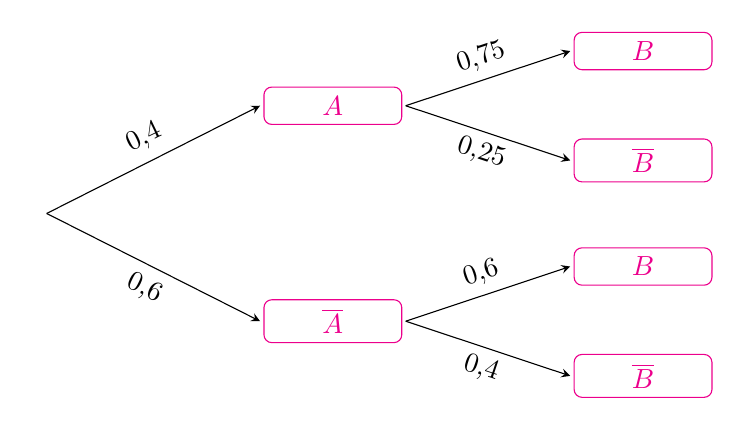
\begin{tikzpicture}
				 \def\gocm{20}
				\def\gocn{10} 
				 \def\r{4}
				\tikzset{s/.style={outer sep=0.5  mm,draw,magenta,rectangle,minimum width=1.75cm,rounded corners=1mm}}
				\path (0,0)  node (O){}++(\gocm:\r) node[s](A1){$A$}++(\gocn:\r) node[s](A2){$B$};
				\path (A1)++({-\gocn}:\r) node[s](a2){$\overline{B}$}; 
				 \path (O)++(-\gocm:\r) node[s](B1){$\overline{A}$}++(\gocn:\r) node[s](B2){$B$};
				\path  (B1)++({-\gocn}:\r) node[s](b2){$\overline{B}$};
				\foreach \x/\y in { 
					 O/A1,A1/A2,
					O/B1,B1/B2, 
					 A1/a2,
					B1/b2} 
				\draw[-stealth](\x.east)--(\y.west); 
				\path  (O)--(A1.west) node[pos=0.5,above,sloped]{$\mbox{0{,}4}$}
					 (O)--(B1.west) node[pos=0.5,below,sloped]{$\mbox{0{,}6}$}
					(B1.east)--(B2.west) node[pos=0.5,above,sloped]{$\mbox{0{,}6}$} 
					 (A1.east)--(A2.west) node[pos=0.5,above,sloped]{$\mbox{0{,}75}$}
					(A1.east)--(a2.west)  node[pos=0.5,below,sloped]{$\mbox{0{,}25}$}
					(B1.east)--(b2.west) node[pos=0.5,below,sloped]{$\mbox{0{,}4}$}; 
			\end{tikzpicture}
	\end{center}
	 \loigiai{
		Ta có $\mathrm{P}  \left(A\right)=\dfrac{4}{10}=0{,}4$; $\mathrm{P} \left(\overline{A}\right)=\dfrac{6}{10}=0{,}6$; $\mathrm{P} \left(B|A\right)=0{,}75$; $\mathrm{P} \left(B|\overline{A}\right)=0{,}6$.\\
		Theo công thức xác suất  toàn phần ta có
		\[\mathrm{P} \left(B\right)=\mathrm{P} \left(A\right) \cdot \mathrm{P}  \left(B|A\right)+\mathrm{P} \left(\overline{A}\right) \cdot \mathrm{P} \left(B|\overline{A}\right)=0{,}4 \cdot 0{,}75+0{,}6 \cdot 0{,}6=0{,}66.\]
	Vậy xác suất để viên đạn trúng mục tiêu  là $0{,}66$.}
\end{bt}

% nguồn: Lop_12_Dai_so_Chuong_6
\begin{bt}%[2D6V2-2]%[ma:eb9ab4ee]
	Trong một trận đấu cờ vua của hai kỳ thủ là Lê Quang Liêm và vua cờ Carlsen; mỗi ván cờ luôn có kẻ thắng người thua (vì nếu hai kỳ thủ hòa thì sẽ bốc thăm để chọn người thắng ván đó). Biết rằng trong mỗi ván đấu, xác suất để anh Liêm dành chiến thắng bằng $0{,}4$; xác suất để Carlsen dành chiến thắng bằng $0{,}6$. Mỗi trận thắng được tính $1$ điểm cho kỳ thủ, người thua không được điểm nào. Nếu người nào tạo được cách biệt $2$ điểm thì sẽ dành chiến thắng chung cuộc. Tính xác suất để Lê Quang Liêm là người chiến thắng sau cùng (làm  tròn đến hàng phần trăm).
	\shortans{0,31} 
	 \loigiai{
		Gọi $\mathrm{P}(n)$ là xác xuất để Lê Quang Liêm dành chiến thắng khi hiệu số điểm của anh so với Carlsen là $n$ điểm, với $n\in \left\{-2;-1; 0; 1;  2\right\}$. \\
		Ta cần tính xác suất chiến thắng của anh Liêm từ trạng thái  $n=0$. \\
		Theo công thức xác suất toàn phần $\mathrm{P}(0)=0{,}4 \cdot  \mathrm{P}(1) + 0{,}6 \times \mathrm{P}(-1)$. \tagEX{1}
		Ta có 
		\begin{itemize}
			\item  $\mathrm{P}(2)=1$.
			\item $\mathrm{P}(-2)=0$. 
			\item $\mathrm{P}(1)=0{,}4 \cdot \mathrm{P}(2)+0{,}6\cdot \mathrm{P}(0)$ hay $\mathrm{P}(1)=0{,}4+0{,}6\cdot \mathrm{P}(0)$. \tagEX{2} 
			\item $\mathrm{P}(-1)=0{,}4 \cdot \mathrm{P}(0)+0{,}6\cdot \mathrm{P}(-2)$ hay $\mathrm{P}(-1)=0{,}4\cdot \mathrm{P}(0)$. \tagEX{3} 
		\end{itemize}
		Thay $(2)$ và $(3)$ vào $(1)$ ta  được
		\[\mathrm{P}(0)=0{,}4\left[0{,}4+0{,}6\cdot \mathrm{P}(0)\right]+0{,}6\cdot 0{,}4\cdot \mathrm{P}(0) \Rightarrow \mathrm{P}(0)=\dfrac{4}{13} \approx 0{,}31.\] 
		Vậy xác suất để Lê Quang Liêm chiến thắng Carlsen  là xấp xỉ $0{,}31$.
	 }
\end{bt}

% nguồn: Lop_12_Dai_so_Chuong_6
\begin{bt}%[2D6V2-2]%[ma:577e7e47]
	Một trường THPT mới thành lập có hai khối $10$ và $11$. Biết tỉ lệ học sinh khối $10$ và khối $11$ là $7:8$. Tỉ lệ học sinh  đạt danh hiệu học sinh khá trở lên của trường là $65\%$ và tỉ lệ này ở khối $11$ là $70\%$. Chọn ngẫu nhiên một học sinh của trường. Tính xác suất học sinh được chọn đạt danh hiệu học sinh khá trở lên của khối $10$. (kết quả làm tròn đến hàng phần trăm)
	\shortans{0,59} 
	\loigiai{ 
		 Gọi $K_{10}$ là biến cố \lq\lq học sinh được chọn thuộc khối $10$\rq\rq.\\
		Gọi $K_{11}$ là biến cố \lq\lq học sinh  được chọn thuộc khối $11$\rq\rq.\\
		Gọi $H$  là biến cố \lq\lq học sinh được chọn đạt danh hiệu học sinh khá trở lên\rq\rq.\\
		Tỉ lệ học sinh khối  $10$ và khối $11$ là $7:8$, tức là\\
		$P(K_{10}) =  \dfrac{7}{7+8} = \dfrac{7}{15}$ và $P(K_{11}) = \dfrac{8}{7+8} = \dfrac{8}{15}$.\\
		Tỉ lệ học sinh đạt danh hiệu học sinh khá trở lên của trường là $65\%$, tức là  $P(H) = 0{,}65$.\\
		Tỉ lệ học sinh đạt danh  hiệu học sinh khá trở lên ở khối $11$ là $70\%$, tức là $P(H|K_{11}) = 0{,}7$.\\
		Ta cần  tính $P(H|K_{10})$.\\
		 Áp dụng công thức xác suất toàn phần:
		\begin{eqnarray*}
			&&P(H) = P(H|K_{10})P(K_{10}) +  P(H|K_{11})P(K_{11})\\
			&\Rightarrow& 0{,}65 = P(H|K_{10}) \cdot \dfrac{7}{15} + 0{,}7 \cdot  \dfrac{8}{15}\\
			&\Rightarrow& P(H|K_{10}) = \dfrac{83}{140}  \approx 0{,}59.
		\end{eqnarray*}
	 }
\end{bt}

% nguồn: Lop_12_Dai_so_Chuong_6
\begin{bt}%[2D6C2-2]%[ma:2064e871]
	Có hai hộp bóng bàn, các quả bóng bàn có kích thước và hình dạng như nhau. Hộp thứ nhất có $3$ quả bóng bàn màu trắng và $2$ quả bóng bàn màu vàng. Hộp thứ hai có $6$ quả bóng bàn màu trắng và $4$ quả  bóng bàn màu vàng. Lấy ngẫu nhiên $4$ quả bóng bàn ở hộp thứ nhất bỏ vào hộp thứ hai rồi lấy ngẫu nhiên $1$ quả bóng bàn ở hộp thứ hai ra. Tính xác suất để lấy được quả bóng bàn màu vàng từ hộp thứ hai (kết quả để dưới dạng số thập phân và làm tròn đến hàng phần chục).
	\shortans{0,4} 
	\loigiai{ 
		Vì hộp thứ nhất có $3$ quả bóng bàn màu trắng và $2$ quả bóng bàn màu vàng nên khi lấy $4$ quả bóng bàn ở hộp thứ nhất thì có hai  khả năng
		\begin{itemize}
			\item Khả năng  thứ nhất là lấy được $3$ quả bóng bàn màu trắng và $1$ quả bóng bàn màu vàng.
			\item Khả năng thứ hai là lấy được $2$ quả bóng bàn màu trắng và $2$ quả bóng bàn  màu vàng.
		\end{itemize}
		Xét các biến cố\\ 
		$A$: \lq\lq Lấy được quả bóng  bàn màu vàng từ hộp thứ hai\rq\rq;\\
		$B$: \lq\lq Lấy được  $4$ quả bóng bàn ở hộp thứ nhất, trong đó có $1$ quả bóng bàn màu vàng\rq\rq;\\
		$\overline{B}$: "Lấy được $4$ quả  bóng bàn ở hộp thứ nhất, trong đó có $2$ quả bóng bàn màu vàng".
		\begin{itemize}
			\item Trường hợp $1$: Số cách lấy $4$ quả bóng bàn từ hộp thứ nhất là $ \mathrm{C}_5^4$, có $1$ cách lấy $3$ quả bóng bàn màu trắng và $2$ cách lấy $1$ quả bóng bàn màu vàng, suy ra $ \mathrm{P}\left(B\right)=\dfrac{1 \cdot 2}{\mathrm{C}_5^4}=\dfrac{2}{5}$.\\ 
			Vì khi đó hộp thứ hai có $9$ quả bóng bàn màu trắng và $5$  quả bóng bàn màu vàng nên $ \mathrm{P} \left(A | B\right)=\dfrac{5}{14}$.
			\item Trường hợp $2$: Số cách lấy $4$ quả bóng bàn từ hộp thứ nhất là $ \mathrm{C}_5^4$, có $ \mathrm{C}_3^2$ cách lấy $2$ quả bóng bàn màu trắng và $1$ cách lấy $2$ quả bóng bàn màu vàng, suy ra $ \mathrm{P}\left(\overline{B}\right)=\dfrac{\mathrm{C}_3^2 \cdot 1}{\mathrm{C}_5^4}=\dfrac{3}{5}$.\\ 
			Vì khi đó hộp thứ hai có $8$ quả bóng bàn màu  trắng và $6$ quả bóng bàn màu vàng nên
			$\mathrm{P} \left(A | \overline{B}\right)=\dfrac{6}{14}$. 
		\end{itemize}
		Theo công thức xác suất toàn phần, ta  có
		$$\mathrm{P}\left(A\right)\text{ =}\mathrm{P}\left(B\right) \cdot \mathrm{P}\left(A | B\right)+\mathrm{P}\left(\overline{B}\right) \cdot  \mathrm{P}\left(A | \overline{B}\right)=\dfrac{2}{5}\cdot\dfrac{5}{14}+\dfrac{3}{5}\cdot\dfrac{6}{14}=0{,}4.$$
	Vậy xác suất để lấy được quả bóng bàn màu vàng từ hộp thứ hai  là $ 0{,}4$.}
\end{bt}

% nguồn: Lop_12_Dai_so_Chuong_6
\begin{bt}%[2D6C2-2]%[ma:47ccdfd3]
	Có một kho bia kém chất lượng chứa các thùng giống nhau ($24$ lon/thùng) gồm $3$ loại: loại $I$ để lẫn mỗi thùng $3$ lon quá hạn sử dụng, loại $II$ để lẫn mỗi thùng $2$ lon quá hạn và loại $III$ để lẫn mỗi thùng có $4$ lon quá hạn. Biết số lượng thùng loại $I$ gấp $2$ lần số lượng thùng loại $II$ và số thùng loại $II$ gấp $3$ lần thùng loại $III$. Chọn ngẫu nhiên $1$ thùng từ trong kho, từ đó chọn ngẫu nhiên $10$ lon. Tính xác suất để lấy được $2$ lon quá hạn sử dụng  (làm tròn đến kết quả phần chục).
	 \shortans{0,3}
	\loigiai{ 
		Gọi $A_i$  là biến cố chọn được thùng loại $i$. $(i=I,II,III)$\\
		$B$ là biến cố chọn  được $10$ sản phẩm trong đó có $2$ lon quá hạn từ thùng được chọn ra.\\
		Gọi số thùng  loại $III$ là $x$ thùng ($x>0$).\\
		Do đó số thùng loại $I$ và loại $II$ lần lượt  là $6x$; $3x$.\\
		Từ đó, ta có $\mathrm{P} \left(A_1\right)=\dfrac{6}{10};\  \mathrm{P} \left(A_2\right)=\dfrac{3}{10};\ \mathrm{P} \left(A_3\right)=\dfrac{1}{10}$.\\
		Xác suất để chọn được thùng có $2$ lon quá  hạn là
		\begin{eqnarray*}
			&& \mathrm{P} \left(B\right) \cdot \mathrm{P} \left(B|A_1 \right)+\mathrm{P} \left(A_2 \right) \cdot \mathrm{P} \left(B|A_2  \right)+\mathrm{P} \left(A_3 \right) \cdot \mathrm{P} \left(B|A_3 \right)\\
			& = &\dfrac{6}{10} \cdot \dfrac{\mathrm{C}_3^2\mathrm{C}_{21}^8}{\mathrm{C}_{24}^{10}}+\dfrac{3}{10} \cdot \dfrac{\mathrm{C}_2^2\mathrm{C}_{22}^8}{\mathrm{C}_{24}^{10}} +\dfrac{1}{10} \cdot \dfrac{\mathrm{C}_4^2\mathrm{C}_{20}^8}{\mathrm{C}_{24}^{10}}  \\
			& \approx  & 0{,}3.
		\end{eqnarray*}
	} 
\end{bt}


%%%%%%%%%%%%%%%% TỰ LUẬN %%%%%%%%%%%%%%%%

% nguồn: Lop_12_Dai_so_Chuong_6
\begin{bt}%[2D6H2-2]%[ma:0703881f]
	Vào mỗi buổi sáng ở tuyến phố X, xác suất xảy ra tắc đường khi trời mưa và không mưa lần lượt là $0{,}6$ và $0{,}3$. Xác suất có mưa vào một buổi  sáng là $0{,}1$. Tính xác suất để sáng đó tuyến phố H bị tắc đường.
	\loigiai{ 
		Gọi $A$ là biến cố \lq\lq Tuyến phố X bị  tắc đường\rq\rq \, và $B$ là biến cố \lq\lq Buổi sáng đó có mưa\rq\rq.\\
		Theo đề ta có $\mathrm{P}\left(B\right)=0{,}1$;  $\mathrm{P}\left(A\mid B\right)=0{,}6$; $\mathrm{P}\left(A\overline{B}\right)=0{,}3$.\\
		Suy ra  $\mathrm{P}\left(\overline{B}\right)= 1-\mathrm{P}\left(B\right)=0{,}9$.\\
		Áp dụng công thức xác suất toàn  phần ta có
		\[\mathrm{P}\left(A\right)=\mathrm{P}\left(B\right)\cdot\mathrm{P}\left(A\mid B\right)+ \mathrm{P}\left(\overline{B}\right)\cdot\mathrm{P}\left(A\overline{B}\right)=0{,}1\cdot0{,}6+0{,}9\cdot0{,}3=0{,}33. 
		 \]
	 }
\end{bt}

% nguồn: Lop_12_Dai_so_Chuong_6
\begin{bt}%[2D6V2-2]%[ma:e1f7c133]
	Trong trò chơi hái hoa có thưởng  của lớp $10$A, cô giáo treo $10$ bông hoa trên cành cây, trong đó có $5$ bông hoa chứa phiếu có thưởng. Bạn Việt hái một bông hoa đầu tiên sau đó bạn Nam hái bông hoa thứ hai. Tính xác suất bạn Nam hái được bông hoa chứa phiếu có thưởng.
	 \loigiai{
		Gọi $A$ là biến cố \lq\lq Bông hoa bạn Nam hái được chứa  phiếu có thưởng\rq\rq \, $B$ là biến cố \lq\lq Bông hoa bạn Việt hái được chứa phiếu có thưởng\rq\rq.\\
		 Ta có $\mathrm{P}\left(B\right)=\dfrac{5}{10}=\dfrac{1}{2}$; $ \mathrm{P}\left(\overline{B}\right)=1-\mathrm{P}\left(B\right)=\dfrac{1}{2}$; $\mathrm{P}\left(A\mid B\right)=\dfrac{4}{9}$; $ \mathrm{P}\left(A\mid \overline{B}\right)=\dfrac{5}{9}$.\\
		Xác suất bạn Nam hái được bông hoa chứa  phiếu có thưởng là
		\[\mathrm{P}\left(A\right)=\mathrm{P}\left(B\right)\cdot\mathrm{P}\left(A\mid B\right)+\mathrm{P}\left(\overline{B}\right) \cdot\mathrm{P}\left(A\mid  \overline{B}\right)=\dfrac{1}{2}\cdot\dfrac{4}{9}+\dfrac{1}{2}\cdot\dfrac{5}{9}=\dfrac{1}{2}.
		 \]
	 }
\end{bt}

% nguồn: Lop_12_Dai_so_Chuong_6
\begin{bt}%[2D6V2-2]%[ma:cc8e962b]
	Tan giờ học buổi chiều một sinh viên có  $60\%$ về nhà ngay, nhưng do giờ cao điểm nên có $30\%$ ngày (số ngày về nhà ngay) bị tắc đường nên bị về nhà muộn. Còn $20\%$ số ngày sinh viên đó vào quán Internet để chơi game, những ngày này xác suất về muộn là $80\%$. Còn lại những ngày khác sinh viên đó đi chơi với bạn bè và những ngày này có xác suất về muộn là $90\%$. Xác suất sinh viên đó về muộn là bao nhiêu?
	\loigiai{ 
		Gọi biến cố $A$:\lq\lq sinh viên đó đi  học về muộn\rq\rq.\\
		Biến cố $B_1$:\lq\lq  sinh viên đó tan học về nhà ngay\rq\rq.\\
		Biến  cố $B_2$:\lq\lq sinh viên đó tan học đi chơi game\rq\rq.\\
		Biến cố $B_3$:\lq\lq  sinh viên đó tan học đi chơi với bạn bè\rq\rq.\\
		Ta có  $\mathrm{P}\left(B_1 \right)=0{,}6$; $\mathrm{P}\left(A\mid B_1 \right)=0{,}3$; $\mathrm{P}\left(B_2 \right)=0{,}2$; $\mathrm{P}\left(A\mid B_2 \right)=0{,}8$; $\mathrm{P}\left(B_3 \right)=0{,}2$; $\mathrm{P}\left(A\mid B_3 \right)=0{,}9$. \\
		Theo công thức xác suất toàn phần, ta có 
		\begin{align*}
			\mathrm{P}\left(A\right)=& \mathrm{P}\left(B_1 \right)\cdot\mathrm{P}\left(A\mid B_1 \right)+\mathrm{P}\left(B_2 \right)\cdot\mathrm{P}\left(A\mid B_2  \right)+\mathrm{P}\left(B_3 \right)\cdot\mathrm{P}\left(A\mid B_3 \right)\\
			=& 0{,}6\cdot0{,}3+0{,}2\cdot 0{,}8+0{,}2\cdot  0{,}9=0{,}52.
		\end{align*}
	} 
\end{bt}

% nguồn: Lop_12_Dai_so_Chuong_6
\begin{bt}%[2D6V2-2]%[ma:ee0758a4]
	Trong một trường học, tỉ lệ học sinh nữ là $52\%$. Tỉ lệ học sinh nữ và tỉ lệ học sinh nam tham gia câu lạc bộ nghệ thuật lần lượt là $18\%$ và $15\%$. Chọn ngẫu nhiên một học sinh của trường. Tính  xác suất học sinh được chọn có tham gia câu lạc bộ nghệ thuật.
	\loigiai{ 
		Gọi $A$ là biến cố \lq\lq Học sinh được chọn là học sinh nữ\rq\rq \, và $B$ là  biến cố \lq\lq Học sinh được chọn tham gia câu lạc bộ nghệ thuật\rq\rq.\\
		Khi đó ta có $\mathrm{P}\left(A\right)=0{,}52$; $\mathrm{P}\left(B\mid A\right)=0{,}18$; $\mathrm{P}\left(B\mid  \overline{A}\right)=0{,}15$.\\
		Suy ra  $\mathrm{P}\left(\overline{A}\right)=1-\mathrm{P}\left(A\right)=0{,}48$.
		Áp dụng công thức xác suất  toàn phần ta có
		\[\mathrm{P}\left(B\right)=\mathrm{P}\left(A\right)\mathrm{P}\left(B\mid  A\right)+\mathrm{P}\left(\overline{A}\right)\mathrm{P}\left(B\mid \overline{A}\right)=0{,}52\cdot 0{,}18+0{,}48\cdot 0{,}15=0{,}1656.
		 \]
	 }
\end{bt}

% nguồn: Lop_12_Dai_so_Chuong_6
\begin{bt}%[2D6V2-2]%[ma:52232cd4]
	Tỉ lệ người dân đã tiêm vắc xin phòng bệnh $A$ ở một địa phương là $65\%$. Trong số những người đã tiêm phòng, tỉ lệ mắc bệnh $A$ là $5\%$; trong số những người chưa tiêm, tỉ lệ mắc bệnh $A$ là $17\%$. Chọn ngẫu nhiên một người ở địa phương đó. Tính xác suất người được chọn mắc  bệnh $A$.
	\loigiai{ 
		Gọi $X$ là biến cố \lq\lq Người  dân được tiêm phòng bệnh $A$\rq\rq \, và
		$Y$ là biến cố \lq\lq Người dân mắc bệnh  $A$\rq\rq. \\
		Ta có  $\mathrm{P}\left(X\right)=0{,}65$; $\mathrm{P}\left(\overline{X}\right)=0{,}35$.\\
		Tỉ lệ mắc  bệnh khi tiêm phòng là $\mathrm{P}\left(Y\mid X\right)=0{,}05$.\\
		Tỉ lệ mắc bệnh khi chưa tiêm  phòng là $\mathrm{P}\left(Y\mid \overline{X}\right)=0{,}17$.\\
		Xác suất người này mắc bệnh $A$ là 
		 \[\mathrm{P}\left(Y\right)=\mathrm{P}\left(X\right)\cdot\mathrm{P}\left(Y\mid X\right)+\mathrm{P}\left(\overline{X}\right)\cdot\mathrm{P}\left(Y\mid \overline{X}\right)=0{,}65\cdot 0{,}05+0{,}35\cdot 0{,}17=0{,}092.\]
	 }
\end{bt}

% nguồn: Lop_12_Dai_so_Chuong_6
\begin{bt}%[2D6V2-2]%[ma:ffd1e1dd]
	Ở một khu rừng nọ có $7$ chú lùn, trong đó có $4$ chú luôn nói thật, $3$ chú còn lại luôn tự nhận mình nói thật nhưng xác suất để mỗi chú này nói thật là $0{,}5$. Bạn Tuyết gặp ngẫu nhiên một chú lùn. Gọi $A$ là biến cố \lq\lq Chú lùn đó  luôn nói thật\rq\rq \, và $B$ là biến cố \lq\lq Chú lùn đó tự nhận mình luôn nói thật\rq\rq. Tính xác suất của các biến cố $A$ và $B$.
	 \loigiai{
		\begin{enumerate}
			\item Ta có, trong $7$ chú lùn thì có $4$ chú  lùn luôn nói thật, nên $\mathrm{P}\left(A\right)=\dfrac{4}{7} \Rightarrow \mathrm{P}\left(\overline{A}\right)=\dfrac{3}{7}$.\\
			Vì $4$ chú lùn luôn nói thật nên $\mathrm{P}\left(B\mid A\right)=1$. 
			 \item Chú lùn còn lại nói thật với xác suất là $0{,}5$ nên ta có $\mathrm{P}\left(B\mid \overline{A}\right)=0{,}5$.\\
			Do đó $\mathrm{P}\left(B\right)=\mathrm{P}\left(A\right)\mathrm{P}\left(B\mid A\right)+\mathrm{P}\left(\overline{A}\right)\cdot\mathrm{P}\left(B\mid \overline{A}\right)=\dfrac{4}{7}\cdot 1+\dfrac{3}{7}\cdot 0{,}5=\dfrac{11}{14}$. 
		\end{enumerate}
	 }
\end{bt}

% nguồn: Lop_12_Dai_so_Chuong_6
\begin{bt}%[2D6V2-2]%[ma:dd773d94]
	Hộp thứ nhất có $3$ viên bi xanh và $6$ viên bi đỏ. Hộp thứ hai có $3$ viên bi xanh và $7$ viên bi đỏ. Các viên bi có cùng kích thước và khối lượng. Lấy ra ngẫu nhiên $1$ viên bi từ hộp thứ nhất chuyển sang hộp thứ hai. Sau đó lại lấy ra ngẫu nhiên đồng thời $2$ viên bi  từ hộp thứ hai. Tính xác suất để hai viên bi lấy ra từ hộp thứ hai là bi đỏ.
	 \loigiai{
		Gọi $A$ là biến cố \lq\lq lấy được một  viên bi màu xanh ở hộp thứ nhất\rq\rq \, và $B$ là biến cố \lq\lq lấy được hai viên bi màu đỏ ở hộp thứ hai\rq\rq.\\
		Khi đó ta có $\mathrm{P}\left(A\right)=\dfrac{1}{3}$,  $\mathrm{P}\left(B\mid A\right)=\dfrac{\mathrm{C}_7^2}{\mathrm{C}_{11}^2}=\dfrac{21}{55}$. \\
		Suy ra $\mathrm{P}\left(\overline{A}\right)=1-\mathrm{P}\left(A\right)=\dfrac{2}{3}$; $\mathrm{P}\left(B\mid \overline{A}\right)=\dfrac{\mathrm{C}_8^2}{\mathrm{C}_{11}^2}=\dfrac{28}{55}$.\\ 
		Áp dụng công thức  xác suất toàn phần ta có
		\[\mathrm{P}\left(B\right)=\mathrm{P}\left(A\right)\mathrm{P}\left(B\mid A\right)+\mathrm{P}\left(\overline{A}\right)\mathrm{P}\left(B\mid  \overline{A}\right)=\dfrac{1}{3}\cdot\dfrac{21}{55}+\dfrac{2}{3}\cdot\dfrac{28}{55}=\dfrac{7}{15}.
		\] 
	 }
\end{bt}

% nguồn: Lop_12_Dai_so_Chuong_6
\begin{bt}%[2D6V2-2]%[ma:223c46ba]
	Một loại linh kiện do hai nhà máy số $I$ và số $II$ cùng sản xuất. Tỉ lệ phế phẩm của các nhà máy $I$ và $II$ lần lượt là $4\%$ và $3\%$ . Trong một lô linh kiện để lẫn lộn $80$ sản phẩm của nhà máy số $I$ và $120$ sản phẩm của nhà máy số $II$. Một khách hàng lấy ngẫu nhiên một linh kiện từ lô hàng đó. Giả  sử linh kiện được lấy ra là linh kiện phế phẩm. Xác suất linh kiện đó do nhà máy nào sản xuất là cao hơn?
	\loigiai{ 
		Xét hai biến cố sau\\ 
		$A$: \lq\lq Linh kiện lấy ra do  nhà máy $I$ sản xuất\rq\rq ,\\
		 $B$: \lq\lq Linh kiện lấy ra là phế phẩm\rq\rq .\\
		Trong lô linh kiện có tổng cộng  $80+120=200$ linh kiện nên $\mathrm{P} \left(A\right)=\dfrac{80}{200}=0{,}4$; $\mathrm{P} \left(\overline{A}\right)=0{,}6$.\\
		Vì tỉ lệ phế phẩm của các nhà máy $I$ và $II$ lần lượt  là $4\%$ và $3\%$ nên $\mathrm{P} \left(B|A\right)=4\%=0{,}04$.\\
		Khi  đó, $\mathrm{P} \left(B|\overline{A}\right)=3\%=0{,}03$ .\\
		Ta có sơ đồ hình  cây
		\begin{center}
			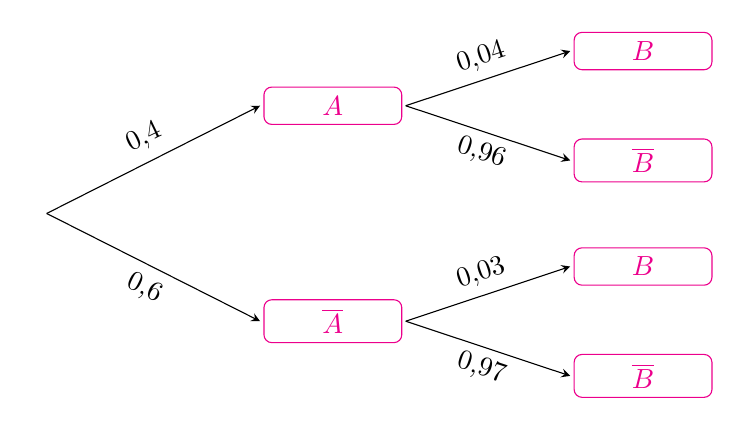
\begin{tikzpicture}
					\def\gocm{20} 
					\def\gocn{10} 
					 \def\r{4}
					 \tikzset{s/.style={outer sep=0.5 mm,draw,magenta,rectangle,minimum width=1.75cm,rounded corners=1mm}}
					\path  (0,0) node (O){}++(\gocm:\r) node[s](A1){$A$}++(\gocn:\r) node[s](A2){$B$};
					\path  (A1)++({-\gocn}:\r) node[s](a2){$\overline{B}$};
					\path (O)++(-\gocm:\r) node[s](B1){$\overline{A}$}++(\gocn:\r)  node[s](B2){$B$};
					\path  (B1)++({-\gocn}:\r) node[s](b2){$\overline{B}$};
					 \foreach \x/\y in {
						O/A1,A1/A2, 
						O/B1,B1/B2, 
						 A1/a2,
						 B1/b2}
					 \draw[-stealth](\x.east)--(\y.west);
					\path (O)--(A1.west) node[pos=0.5,above,sloped]{$\mbox{0{,}4}$} 
						(O)--(B1.west)  node[pos=0.5,below,sloped]{$\mbox{0{,}6}$}
						 (B1.east)--(B2.west) node[pos=0.5,above,sloped]{$\mbox{0{,}03}$}
						 (A1.east)--(A2.west) node[pos=0.5,above,sloped]{$\mbox{0{,}04}$}
						(A1.east)--(a2.west)  node[pos=0.5,below,sloped]{$\mbox{0{,}96}$}
						(B1.east)--(b2.west) node[pos=0.5,below,sloped]{$\mbox{0{,}97}$}; 
				\end{tikzpicture}
		\end{center}
		Khi linh kiện lấy ra là phế phẩm thì xác suất linh kiện đó do nhà máy $I$ sản xuất là $\mathrm{P}\left(A|B\right)$ và xác suất linh kiện đó do  nhà máy $II$ sản xuất là $\mathrm{P}\left(\overline{A}|B\right)$ .\\
		Áp dụng công thức Bayes, ta  có
		$$\mathrm{P} \left(A|B\right)=\dfrac{\mathrm{P} \left(A\right) \cdot  \mathrm{P}\left(B|A\right)}{\mathrm{P}\left(A\right) \cdot \mathrm{P}\left(B|A\right)+\mathrm{P} \left(\overline{A}\right) \cdot \mathrm{P} \left(B|\overline{A}\right)}=\dfrac{0{,}4 \cdot 0{,}04}{0{,}4 \cdot 0{,}04+0{,}6 \cdot 0{,}03}\approx 47\%.$$
		Suy ra $\mathrm{P} \left(\overline{A}|B\right)=1-\mathrm{P}  \left(A|B\right)\approx 53\%$.\\
		Vậy xác suất linh kiện đó do  nhà máy $II$ sản xuất là cao hơn.
	 }
\end{bt}

% nguồn: Lop_12_Dai_so_Chuong_6
\begin{bt}%[2D6V2-2]%[ma:b64a2f1b]
	Có hai cái hộp. Hộp thứ nhất có $4$  bi trắng và $5$ bi đen. Hộp thứ hai có $5$ bi trắng và $4$ bi đen. Chọn ngẫu nhiên $3$ viên bi ở hộp thứ nhất bỏ vào hộp thứ hai rồi sau đó chọn ngẫu nhiên $1$ viên bi ở hộp thứ hai. Khi đó xác suất để lấy được bi trắng là bao nhiêu?
	\loigiai{ 
		Gọi $B_k$ là biến cố \lq\lq  lấy ra được $k$ viên bi trắng từ hộp thứ nhất\rq\rq \, trong đó $k=0, 1, 2, 3$.\\
		Gọi $A$ là biến cố \lq\lq lấy được viên bi  trắng từ hộp thứ hai\rq\rq. Khi đó
		\begin{itemize}
			\item Xác suất lấy ra được $0$  viên bi trắng từ hộp thứ nhất là $\mathrm{P}\left(B_0 \right)=\dfrac{\mathrm{C}_5^3}{\mathrm{C}_9^3}=\dfrac{5}{42}$.
			\item Xác suất lấy ra  được $1$ viên bi trắng từ hộp thứ nhất là $\mathrm{P}\left(B_1 \right)=\dfrac{\mathrm{C}_4^1\mathrm{C}_5^2}{\mathrm{C}_9^3}=\dfrac{10}{21}$.
			 \item Xác suất lấy ra được $2$ viên bi trắng từ hộp thứ nhất là $\mathrm{P}\left(B_2 \right)=\dfrac{\mathrm{C}_4^2\mathrm{C}_5^1}{\mathrm{C}_9^3}=\dfrac{5}{14}$.
			\item Xác suất lấy ra được $3$ viên  bi trắng từ hộp thứ nhất là $\mathrm{P}\left(B_2 \right)=\dfrac{\mathrm{C}_4^3}{\mathrm{C}_9^3}=\dfrac{1}{21}$.
			\item Xác  suất lấy được $1$ bi trắng từ hộp thứ hai với điều kiện lấy được $0$ bi trắng từ hộp thứ nhất là
			$\mathrm{P}\left(A\mid B_0 \right)=\dfrac{5}{12}$. 
			\item Xác suất lấy được $1$ bi trắng từ hộp  thứ hai với điều kiện lấy được $1$ bi trắng từ hộp thứ nhất là
			 $\mathrm{P}\left(A\mid B_1 \right)=\dfrac{6}{12}=\dfrac{1}{2}$.
			\item Xác suất lấy được $1$ bi trắng từ hộp thứ hai với điều kiện lấy được $2$ bi trắng từ hộp  thứ nhất là
			$\mathrm{P}\left(A\mid B_2  \right)=\dfrac{7}{12}$.
			\item Xác suất lấy được $1$ bi trắng từ hộp thứ hai  với điều kiện lấy được $3$ bi trắng từ hộp thứ nhất là
			 $\mathrm{P}\left(A\mid B_3 \right)=\dfrac{8}{12}=\dfrac{2}{3}$.
		\end{itemize}
		Theo công thức xác suất toàn phần, ta có 
		\[\mathrm{P}\left(A\right)=\mathrm{P}\left(B_0 \right)\cdot\mathrm{P}\left(A\mid B_0 \right)+\mathrm{P}\left(B_1 \right)\cdot\mathrm{P}\left(A\mid B_1 \right)+\mathrm{P}\left(B_2  \right)\cdot\mathrm{P}\left(A\mid B_2 \right)+\mathrm{P}\left(B_3 \right)\cdot\mathrm{P}\left(A\mid B_3 \right)=\dfrac{19}{36}.
		 \]
		Vậy xác suất để  lấy được bi trắng từ hộp thứ hai theo đề bài trên là $\dfrac{19}{36}$.
	 }
\end{bt}

% nguồn: Lop_12_Dai_so_Chuong_6
\begin{bt}%[2D6V2-2]%[ma:3b31ddfb]
	Một công ty  một ngày sản xuất được $850$ sản phẩm trong đó có $50$ sản phẩm không đạt chất lượng. Lần lượt lấy ra ngẫu nhiên không hoàn lại $2$ sản phẩm để kiểm tra. Xác suất để sản phẩm thứ hai không đạt chất lượng là bao nhiêu?
	 \loigiai{
		Gọi $A_1$, $A_2$ lần lượt là các biến  cố sản phẩm thứ nhất, sản phẩm thứ hai không đạt chất lượng.\\
		Nếu sản phẩm thứ nhất không đạt chất lượng thì còn $49$ sản phẩm không đạt chất lượng trong tổng số  $849$ sản phẩm nên $\mathrm{P}\left(A_2\mid A_1 \right)=\dfrac{49}{849}$.\\
		Ta có $\mathrm{P}\left(A_1  \right)=\dfrac{50}{850}$, $ \mathrm{P}\left(\overline{A_1}\right)=\dfrac{800}{850}$ và $\mathrm{P}\left(A_2\mid \overline{A_1}\right)=\dfrac{50}{849}$.\\
		Xác suất  để sản phẩm thứ hai không đạt chất lượng là
		\[\mathrm{P}\left(A_2 \right)=\mathrm{P}\left(A_1  \right)\cdot\mathrm{P}\left(A_2\mid A_1 \right)+\mathrm{P}\left(\overline{A_1}\right)\cdot\mathrm{P}\left(A_2\mid \overline{A_1}\right)=\dfrac{50}{850}\cdot\dfrac{49}{849}+\dfrac{800}{850}\cdot\dfrac{50}{849}=\dfrac{1}{17}.
		 \]
	} 
\end{bt}

% nguồn: Lop_12_Dai_so_Chuong_6
\begin{bt}%[2D6V2-2]%[ma:df6e70b4]
	Một chiếc hộp có $80$ viên bi, trong đó  có $50$ viên bi màu đỏ và $30$ viên bi màu vàng; các viên bi có kích thước và khối lượng như nhau. Sau khi kiểm tra, người ta thấy có $60\%$ số viên bi màu đỏ đánh số và $50\%$ số viên bi màu vàng có đánh số, những viên bi còn lại không đánh số. Lấy ra ngẫu nhiên một viên bi trong hộp. Tính xác suất để viên bi được lấy ra có đánh số.
	 \loigiai{
		Gọi $A$ là biến cố \lq\lq viên bi được lấy ra có đánh số\rq\rq; $B$ là biến cố \lq\lq viên bi  được lấy ra có màu đỏ\rq\rq.
		 suy ra $\overline{B}$ là biến cố \lq\lq viên bi được lấy ra có màu vàng\rq\rq.\\
		Xác suất để viên bi được  lấy ra có đánh số là $\mathrm{P}\left(A\right)=\mathrm{P}\left(B\right)\cdot\mathrm{P}\left(A\mid B\right)+\mathrm{P}\left(\overline{B}\right)\cdot\mathrm{P}\left(A\mid \overline{B}\right)$.\\
		 Ta có $\mathrm{P}\left(B\right)=\dfrac{50}{80}=\dfrac{5}{8}$, $ \mathrm{P}\left(\overline{B}\right)=\dfrac{30}{80}=\dfrac{3}{8}$, $ \mathrm{P}\left(A\mid B\right)=60\%=\dfrac{3}{5}$, $ \mathrm{P}\left(A\mid \overline{B}\right)=50\%=\dfrac{1}{2}$.\\
		Do đó  $\mathrm{P}\left(A\right)=\mathrm{P}\left(B\right) \cdot \mathrm{P}\left(A\mid B\right)+\mathrm{P}\left(\overline{B}\right) \cdot \mathrm{P}\left(A\mid \overline{B}\right)=\dfrac{5}{8}\cdot\dfrac{3}{5}+\dfrac{3}{8}\cdot\dfrac{1}{2}=\dfrac{9}{16}$.
	 }
\end{bt}

% nguồn: Lop_12_Dai_so_Chuong_6
\begin{bt}%[2D6V2-2]%[ma:79dc5064]
	Một nhà máy sản xuất điện thoại có hai dây chuyền sản xuất $I$ và $II$. Sản phẩm điện thoại di động được sản xuất của dây chuyền $I$ chiếm $70\%$ còn điện thoại di động được sản xuất dây chuyền $II$ chiếm $30\%$ tổng sản phẩm của công ty. Tỉ lệ sản phẩm bị lỗi của dây chuyền $I$ chiếm $2\%$ còn của dây chuyền $II$ chiếm $3\%$ tổng sản phẩm công ty. Giả sử một chiếc điện thoại di động ngẫu nhiên được kiểm tra và phát hiện bị lỗi. Tính xác suất chiếc điện thoại này được sản xuất bởi dây chuyền  $I$.
	Gọi $A$ là biến cố \lq\lq Sản phẩm bị lỗi\rq\rq.\\ 
	Gọi $B$ là biến cố \lq\lq Điện thoại được chọn do dây  chuyền $I$ sản xuất \rq\rq .\\
	Suy ra $\overline{B}$ là biến cố \lq\lq Điện thoại được chọn do dây chuyền  $II$ sản xuất \rq\rq .\\
	Ta có $\mathrm{P} \left(B\right)=0{,}7$ và $\mathrm{P} \left(\overline{B}\right)=1-0{,}7=0{,}3$; $\mathrm{P}  \left(A|B\right)=0{,}02$ và $\mathrm{P} \left(A|\overline{B}\right)=0{,}03$.\\
	 Khi đó xác suất để điện thoại được chọn ra bị lỗi là
	\[\mathrm{P} \left(A\right)=\mathrm{P} \left(B\right) \cdot \mathrm{P}\left(A|B\right)+\mathrm{P}  \left(\overline{B}\right) \cdot \mathrm{P} \left(A|\overline{B}\right)=0{,}7 \cdot 0{,}02+0{,}3 \cdot 0{,}03=0{,}023.\]
	Do điện thoại lấy  ra bị lỗi nên xác suất điện thoại đó do dây chuyền $I$ sản xuất là\\
	\[\mathrm{P} \left(B|A\right)=\dfrac{\mathrm{P} \left(B\right) \cdot \mathrm{P}\left(A|B\right)}{\mathrm{P}\left(A\right)}=\dfrac{0{,}7  \cdot 0{,}02}{0{,}023}=\dfrac{14}{23}.\]
	Vậy xác suất một chiếc điện  thoại bị lỗi được sản xuất bởi dây chuyền $I$ là khoảng $60{,}87\%$.
\end{bt}
